%\documentclass[preprint,letterpaper,floatfix,citeautoscript,aip,jcp]{revtex4-1}
%
%\usepackage{fullpage}
%\usepackage{amsfonts}
%\usepackage{graphicx}
%\usepackage{amsmath}
%\usepackage{chemfig}
%\usepackage{indentfirst}

%\documentclass[12pt]{article}
%\documentclass[letterpaper,floatfix,citeautoscript,aip,jcp]{revtex4-1}
%\documentclass[letterpaper,floatfix,citeautoscript,showkeys]{revtex4-1}
%\documentclass[twocolumn,letterpaper,floatfix,citeautoscript,jcp]{revtex4-1}
%\documentclass[twocolumn,letterpaper,floatfix,citeautoscript,aip,jcp]{revtex4-1}
\documentclass[journal=jctc,manuscript=article]{achemso}
\setkeys{acs}{maxauthors=30,etalmode=truncate}
%%%%%%%%%%%%%%%%%%%%%%%%%%%%%%%%%%%%%%%%%%%%%%%%%%%%%%%%%%%%%%%%%%%%%
%% Place any additional packages needed here.  Only include packages
%% which are essential, to avoid problems later.
%%%%%%%%%%%%%%%%%%%%%%%%%%%%%%%%%%%%%%%%%%%%%%%%%%%%%%%%%%%%%%%%%%%%%
\usepackage{chemformula} % Formula subscripts using \ch{}
\usepackage[T1]{fontenc} % Use modern font encodings

%%%%%%%%%%%%%%%%%%%%%%%%%%%%%%%%%%%%%%%%%%%%%%%%%%%%%%%%%%%%%%%%%%%%%
%% If issues arise when submitting your manuscript, you may want to
%% un-comment the next line.  This provides information on the
%% version of every file you have used.
%%%%%%%%%%%%%%%%%%%%%%%%%%%%%%%%%%%%%%%%%%%%%%%%%%%%%%%%%%%%%%%%%%%%%
%%\listfiles

%%%%%%%%%%%%%%%%%%%%%%%%%%%%%%%%%%%%%%%%%%%%%%%%%%%%%%%%%%%%%%%%%%%%%
%% Place any additional macros here.  Please use \newcommand* where
%% possible, and avoid layout-changing macros (which are not used
%% when typesetting).
%%%%%%%%%%%%%%%%%%%%%%%%%%%%%%%%%%%%%%%%%%%%%%%%%%%%%%%%%%%%%%%%%%%%%
% \newcommand*\mycommand[1]{\texttt{\emph{#1}}}

\usepackage{fullpage}
\usepackage{amsfonts}
\usepackage{graphicx}
\usepackage{float}
\usepackage{amsmath}
\usepackage{chemfig}
\usepackage{indentfirst}
\usepackage{longtable}
\usepackage{array}
\usepackage{cellspace}
\usepackage{palatino}
%\usepackage{breqn}
\usepackage{amssymb}
\usepackage{verbatim}
\usepackage[colorlinks=true,citecolor=blue,linkcolor=blue]{hyperref}
\usepackage{siunitx}
\usepackage{xr}

\makeatletter
\newcommand*{\addFileDependency}[1]{% argument=file name and extension
	\typeout{(#1)}
	\@addtofilelist{#1}
	\IfFileExists{#1}{}{\typeout{No file #1.}}
}
\makeatother

\newcommand*{\myexternaldocument}[1]{%
	\externaldocument{#1}%
	\addFileDependency{#1.tex}%
	\addFileDependency{#1.aux}%
}

%\myexternaldocument{H:/property_estimation/Supporting_Information_JCTC_pre_BERB}

\SectionNumbersOn

% The figures are in a figures/ subdirectory.
\graphicspath{{figures/}}

%\bibliographystyle{apsrevlong}
%\bibliographystyle{apsrev}
\bibliographystyle{unsrt}

% italicized boldface for math (e.g. vectors)
\newcommand{\bfv}[1]{{\mbox{\boldmath{$#1$}}}}
% non-italicized boldface for math (e.g. matrices)
\newcommand{\bfm}[1]{{\bf #1}}          

%\newcommand{\bfm}[1]{{\mbox{\boldmath{$#1$}}}}
%\newcommand{\bfm}[1]{{\bf #1}}
\newcommand{\expect}[1]{\left \langle #1 \right \rangle} % <.> for denoting expectations over realizations of an experiment or thermal averages

\newcommand{\var}[1]{{\mathrm var}{(#1)}}
\newcommand{\x}{\bfv{x}}
\newcommand{\y}{\bfv{y}}
\newcommand{\f}{\bfv{f}}

\newcommand{\hatf}{\hat{f}}

\newcommand{\bTheta}{\bfm{\Theta}}
\newcommand{\btheta}{\bfm{\theta}}
\newcommand{\bhatf}{\bfm{\hat{f}}}
\newcommand{\Cov}[1] {\mathrm{cov}\left( #1 \right)}
\newcommand{\T}{\mathrm{T}}                                % T used in matrix transpose

\newcommand\blfootnote[1]{%
	\begingroup
	\renewcommand\thefootnote{}\footnote{#1}%
	\addtocounter{footnote}{-1}%
	\endgroup
}

\title{United-atom, Mie $\lambda$-6 force fields for normal and branched alkanes extrapolate poorly to high pressures when parameterized using vapor-liquid equilibria properties. To be submitted to the Journal of Physical Chemistry, B.}
%Alternative titles: Impact of repulsive exponent on high pressure systems
%MRS1: suggestion: make the title the conclusion?  Such as ``Baysian inference shows that Mie-6 united atom force fields cannot predict vapor-liquid equilibria for alkanes?'' or ``Mie-6 united atom force fields cannot predict thermophysical properties of alkanes at high pressure''? I've had success with such straightforward titles; people know what they are getting, and get those answers when they google the question.
% Bayesian inference demonstrates limitations at high pressures of transferable, united-atom, Mie $\lambda$-6 force fields for normal and branched alkanes
% Bayesian inference analysis of transferable, united-atom, Mie $\lambda$-6 force fields for normal and branched alkanes.
%Bayesian inference demonstrates limitations for predicting vapor-liquid equilibria and high pressures that united-atom, Mie $\lambda$-6 force fields for normal and branched alkanes.
%Bayesian inference demonstrates that united-atom, Mie $\lambda$-6 force fields extrapolate poorly to high pressures when parameterized using vapor-liquid equilibria properties.
%Bayesian inference demonstrates limitations of united-atom, Mie $\lambda$-6 force fields for predicting both vapor-liquid equilibria properties and high pressures of normal and branched alkanes.
%United-atom, Mie $\lambda$-6 force fields for normal and branched alkanes extrapolate poorly to high pressures when parameterized using vapor-liquid equilibria properties.

\author{Richard A. Messerly}
\email{richard.messerly@nist.gov}
\affiliation{Thermodynamics Research Center, National Institute of Standards and Technology, Boulder, Colorado, 80305}

\author{Michael R. Shirts}
\email{michael.shirts@colorado.edu}
\affiliation{Department of Chemical and Biological Engineering, University of Colorado, Boulder, Colorado, 80309}

\author{Andrei F. Kazakov}
\email{andrei.kazakov@nist.gov}
\affiliation{Thermodynamics Research Center, National Institute of Standards and Technology, Boulder, Colorado, 80305}

\keywords{Transferability, Molecular Dynamics, Molecular Simulation, Monte Carlo, Markov Chain, Bayesian Inference}%Use showkeys class option if keyword

\begin{document}
	
\blfootnote{Contribution of NIST, an agency of the United States government; not subject to copyright in the United States.}

\begin{abstract}

\end{abstract}

\maketitle

\section*{Purpose}

%The aim of this study is to demonstrate, using Bayesian inference, that a UA Mie force field cannot adequately predict VLE and PVT of compressed liquids and supercritical fluids for normal and branched alkanes. For adequate prediction of VLE and compressed liquid pressures, we recommend using AUA or AA models. % or perhaps Exp-6 or extended Lennard-Jones, i.e. 12-10-8-6. %We then use simple Bayes factors (if not RJMC) to determine the optimal value of lambda for predicting compressed liquid pressures. 
%%%% RAM: Andrei and I think that we don't really need to find the best lambda value since most people would not be willing to sacrifice Pvsat just to match high pressures. Also Andrei wants to minimize the amount of effort/time required to get this paper ready.
%%%% MRS: ``since most people would not be willing to sacrifice Pvsat'': right, then just state the reasonings for not including it, that you don't think people would care.
%MRS: is it just VLE at high pressures, or everywhere?
%\section*{Outline}
%MRS: if no data on 12-10-8-6, don't recommend.
%MRS: if you say people should use AUA, then the questions is whether you need to do simulations.  It depends what the current thinking on the field is.  If AUA and Mie are thought to work, then showing that Mie doesn't is sufficient for the thesis.

%%% These were some of my thoughts before meeting with Andrei. Skip this section.

%\begin{enumerate}
%	\item Introduction
%	\item Bayesian Theory
%	\begin{enumerate}
%		\item Posterior
%		\item MCMC
%		\item RJMC
%	\end{enumerate}
%    \item MBAR-ITIC
%    \item Simulation details
%    \item Force field
%	\item Lambda (RJMC)
%	\item Transferability of CH2 sites
%	\item Transferability of CH3 sites using RJMC
%	\item Combining rules (RJMC)
%	\item Viscosity PoU
%	\item Higher pressure PoU
%\end{enumerate}
%
%Are we justified in picking just a single value for lambda? Or should we have a range of lambda values?
%Are we justified in fitting CH3 and CH2 sites simultaneously?
%Is one combining rule favored over another?
%
%I think for this paper we could focus on just a couple of these points. RJMC needs to be working for some of these. Lambda I could probably do without RJMC. Same with CH2. But others it would be necessary. 
%I basically already have the results for lambda (just ethane) and for the CH2 sites.
%
%Oh, for CH2 I could use RJMC to see if we should have a single CH2 site or if we need to have a CH2 for each. Basically I would have the same posterior (combined for all three) and I would have the model choose between the same and different. Right?
%
%So if I develop surrogate models for logp, I could perform this analysis very quickly. Then if I develop them for rhol, Psat I can change the likelihood function. For now though I am just going to use logp.
%
%Several decisions are made somewhat arbitrarily when developing force fields...
%
%I can perform a simple Bayesian inference analysis and show how the Mie potential cannot accurately predict VLE and high pressure PVT
%I could just perform this analysis for the 16-6 potential, since I already have that all done for n-alkanes
%I can show how TraPPE and Potoff perform to show the opposite trends of the 12-6 and 16-6
%Then show how the uncertainty in epsilon and sigma cannot reconcile this for the 16-6
%Then show how even a 15-6 or 14-6 potential cannot match all three properties
%
%The goal of this study is to determine if there exists a set of eps, sig, lam that accurately predicts VLE and supercritical PVT
%Specifically, we are testing whether or not the UA approach can adequately predict high pressure densities
%
%We can show how TraPPE-UA2 and/or TAMie does a better job at high pressures
%I could also simulate Exp-6

%\begin{enumerate}
%	\item Introduction
%	\item Methods I
%	\begin{enumerate}
%		\item Simulation details
%		\item Force field
%	\end{enumerate}
%	\item Case Study for alkanes
%	\item Methods II
%	\begin{enumerate}
%		\item Bayesian Analysis
%		\item Surrogate Model
%		\item Propagation of Uncertainty
%		%%%% RAM: Do we want to consider performing a Pareto front analysis to show that no set of eps, sig, lam can match all three? %%%%
%                %%%% MRS: probably would be good; I don't think it would require performing additional simulations? Also, bec clear which three properties.   
%	\end{enumerate}
%	\item Results
%	\begin{enumerate}
%		\item VLE and Compressed
%		\begin{enumerate}
%			\item Parameter uncertainties
%			\item Propagation of uncertainties
%		\end{enumerate}
%	    %\item Optimal $\lambda$ for high pressures %%% RAM: This distracts from the main purpose, that the Mie potential cannot match all three properties %%%MRS: keep it simple.
%	\end{enumerate}
%	\item Future Work
%	\item Conclusions	
%\end{enumerate}

%	\item Higher pressure PoU
%	\item Different values of lambda cannot reconcile (already done for ethane, probably need to do for other alkanes)
%	\item AUA, AUA Mie, Exp-6

%\section*{Detailed Outline}

\section{Introduction}

An accurate understanding of the relationship between pressure, volume (or density, $\rho$), and temperature $(PVT)$ and caloric properties (such as heat capacity) for a given compound is essential for designing industrial chemical processes. Fundamental equations of state (FEOS), such as those based on the Helmholtz free energy, are a powerful approach for estimating $PVT$ behavior and caloric properties. For example, the National Institute of Standards and Technology (NIST) REFPROP (Reference Fluid Properties) currently provides FEOS for around one hundred chemical species \cite{LEMMON-RP91}. Unfortunately, most compounds do not have sufficient (reliable) experimental data covering a wide range of pressures, densities, and temperatures to develop a highly-accurate FEOS. Using an FEOS to extrapolate to temperatures and pressures that are significantly higher than those used in parameterizing the FEOS can result in large errors. Therefore, improvement in an FEOS at high temperatures and pressures necessitates additional data near those conditions.
% Most compounds do not have sufficient reliable experimental data over a wide enough region of phase space. 
%However, Thol et al. demonstrated that molecular simulation results at high temperatures and pressures can be used to supplement experimental data when developing fundamental equations of state \cite{Thol2016_siloxane}.
%Unfortunately, most compounds do not have sufficient (reliable) experimental data covering a wide range of pressures, densities, and temperatures are required to develop a highly-accurate FEOS, but are not available for most compounds.

The lack of experimental data at high temperatures and pressures, especially, is likely attributed to the inherent safety, cost, and complexity of such experiments. By contrast, molecular simulation (i.e. Monte Carlo, MC, and molecular dynamics, MD) methods at high temperatures and pressures do not suffer from any of these limitations. Therefore, in principle, molecular simulation could aid in developing FEOS  \cite{Thol2016_LJ,Thol_LJTS,Rutkai2017,Lustig2015,Rutkai2013,Rutkai2015}. For example, several recent studies by Thol et al. supplement experimental data with molecular simulation results at temperatures and pressures beyond the range of available experimental temperatures and pressures \cite{Thol2016_siloxane_first,Thol2016_siloxane,Thol2017}. Specifically, experimental data were available for temperatures and pressures up to 580 K and 130 MPa, 590 K and 180 MPa, and 560 K and 100 MPa for hexamethyldisiloxane, octamethylcyclotetrasiloxane, and 1,2-dichloroethane, respectively. Molecular simulations were performed for these compounds at temperatures and pressures up to 1200 K and 600 MPa, 1200 K and 520 MPa, 1000 K and 1200 MPa, respectively. The inclusion of these simulation results improved the performance of the FEOS at extreme temperatures and pressures. 

%Typically, force fields are parameterized with vapor-liquid equilibria data

Hydrocarbons are a fundamental feed-stock for many petrochemical processes and, therefore, large amounts of experimental data exist covering a wide range of $PVT$ phase space. For these reasons, REFPROP contains highly-accurate FEOS for several hydrocarbons, most of which are shorter-chains (less than 20 carbons) with limited branching (i.e. only methyl branches). An appealing approach to develop FEOS for other hydrocarbons, is to utilize hybrid data sets consisting of experimental data and molecular simulation results at extreme temperatures and pressures. 

The primary limitation for implementing molecular simulation at extreme temperatures and pressures is whether or not the force field, which is typically parameterized using VLE data, is reliable at those conditions, i.e. if the VLE optimal parameters are transferable to higher temperatures and pressures. In this study, we investigate how well the traditional force fields for predicting VLE extrapolate to higher temperatures (supercritical fluid) and pressures (compressed liquid). This analysis is performed for four normal and four branched alkanes by comparing the simulated compressibility factor $(Z)$ with the REFPROP correlations, which are assumed to be reliable at these conditions.

The most accurate force fields for estimating hydrocarbon VLE properties (i.e. $\rho_{\rm l}^{\rm sat}$ and $P_{\rm v}^{\rm sat}$) are Transferable Potentials for Phase Equilibria (TraPPE) \cite{TraPPE,Martin1999} (and, especially, the recent TraPPE-2 \cite{TraPPEUA2}), Errington \cite{Exp6}, anisotropic-united-atom (AUA4) \cite{AUA4,Bourasseau2002}, Potoff \cite{Mie,Potoff_branched}, and Transferable anisotropic Mie potential (TAMie) \cite{TAMie,Weidler2016}. The TraPPE and Potoff force fields use a united-atom (UA) model while the TraPPE-2, Errington, AUA4, and TAMie force fields use an anisotropic-united-atom (AUA) model. Both a UA and AUA model group the hydrogen interactions with their neighboring carbon atom. However, the UA model assumes that the UA interaction site is that of the carbon atom, while an AUA model assumes that the AUA interaction site is shifted away from the carbon atom and towards the hydrogen atom(s). Although, in theory, an all-atom (AA) force field should yield more accurate results, from a parameterization standpoint, it is much easier to ensure that a global minimum is obtained when parameterizing UA and AUA force fields since fewer parameters are optimized simultaneously. The reduced computational cost is an additional benefit of the UA and AUA approach.

%
%implicit hydrogens (IH) instead of explicit hydrogens (EH). An IH model does not directly compute the hydrogen interactions, rather the hydrogens are grouped with their neighboring carbon atom. The two classes of IH models are united-atom (UA) and anisotropic-united-atom (AUA). A UA model assumes that the UA interaction site is that of the carbon atom, while a AUA model assumes that the AUA interaction site is shifted away from the carbon atom and towards the hydrogen atom(s). Although, in theory, an all-atom (AA) force field should yield more accurate results, from a parameterization standpoint, it is much easier to ensure that a global minimum is obtained when optimizing UA and AUA force fields. The reduced computational cost is an additional benefit of the UA and AUA approach.
%
%Several literature UA and AUA force fields have been optimized to agree with VLE properties for normal and branched alkanes. Two of the most widely used UA based force fields are the TraPPE LJ 12-6 and Potoff Mie 16-6, while two of the most successful AUA force fields are the AUA4 LJ 12-6 and TAMie Mie 14-6. 

In addition to the classification of UA and AUA force fields, the existing force fields differ in the non-bonded functional form and corresponding parameters. The TraPPE, TraPPE-2, and AUA4 force fields use a Lennard-Jones (LJ) 12-6 potential, while the Potoff and TAMie force fields use the Mie $\lambda$-6 (or generalized Lennard-Jones) potential, and the Errington force field uses the Buckingham exponential-6 (Exp-6) potential. The three-parameter Mie $\lambda$-6 and Exp-6 potentials are more flexible than the two-parameter LJ 12-6 potential as the additional adjustable parameter controls the steepness of the repulsive barrier.

% have three adjustable parameters while the LJ 12-6 potential only has two parameters.

Previous work demonstrated that the UA LJ 12-6 potential cannot adequately estimate both $\rho_{\rm l}^{\rm sat}$ and $P_{\rm v}^{\rm sat}$ for \textit{n}-alkanes \cite{Pareto_LJPQ,Mess4}. For this reason, the TraPPE-UA force field was primarily developed to agree with saturated liquid densities \cite{TraPPE}. By contrast, accurate prediction of both $\rho_{\rm l}^{\rm sat}$ and $P_{\rm v}^{\rm sat}$ over a wide temperature range is possible by varying the repulsive exponent of the LJ potential (i.e. the Mie $\lambda$-6 potential). Typically, the optimal value of $\lambda$ is greater than 12 with a corresponding increase in the well depth $(\epsilon)$. Specifically for hydrocarbons, the Potoff UA force field uses $\lambda = 16$ while the TAMie force field uses $\lambda = 14$. However, there is some concern that increasing the repulsive exponent might have some undesirable consequences, especially at high pressures, where close range interactions will become more prevalent than at vapor-liquid equilibria. The purpose of this study is to determine whether or not the UA Mie potential is adequate for predicting both VLE and PVT at higher temperatures and pressures. 

The outline for this manuscript is the following. Section \ref{Methods I} discusses the simulation and force field details. Section \ref{Case Study} is a case study for normal and branched alkanes using the existing force fields developed from VLE properties. Section \ref{Methods II} explains how Bayesian inference is employed to investigate the adequacy of the UA Mie potential. Section \ref{Results} presents the results from the Bayesian analysis. Section \ref{Conclusions} reports the primary conclusions of this study.

%when properly optimized, the Mie potential can accurately predict both $\rho_{\rm l}^{\rm sat}$ and $P_{\rm v}^{\rm sat}$ over a wide temperature range. This improvement  However, there is some concern that increasing the repulsive exponent (in this case, from 12 to 16) might have some undesirable consequences, especially at high pressures, where close range interactions will become more significant. The purpose of this study is to determine whether or not the UA Mie potential is 
%
%are reliable at high temperatures and pressure
%
%Several 
%
%Although, in theory, an all-atom (AA) force field would be more reliable than a UA and AUA force field, from a parameterization standpoint, it is much easier to ensure that a global minimum is obtained when optimizing UA and AUA force fields.
%
%The most reliable hydrocarbon force fields for estimating VLE properties (i.e. $\rho_{\rm l}^{\rm sat}$ and $P_{\rm v}^{\rm sat}$) are based on the united-atom (UA) assumption, where hydrogen interactions are grouped with their neighboring carbon atom, or the anisotropic-united-atom (AUA) model, where the hydrogens  force fields are typically considered 
%
%Hydrocarbons 
%
%Several force fields in the literature have been optimized to agree with VLE properties for normal and branched alkanes. Two of the most widely used united-atom based force fields are the TraPPE LJ 12-6 and Potoff Mie 16-6.
%
%It has been demonstrated that the united-atom LJ 12-6 potential cannot adequately estimate both $\rho_{\rm l}^{\rm sat}$ and $P_{\rm v}^{\rm sat}$. By contrast, when properly optimized, the Mie 16-6 potential can accurately predict both $\rho_{\rm l}^{\rm sat}$ and $P_{\rm v}^{\rm sat}$ over a wide temperature range. However, there is some concern that increasing the repulsive exponent (in this case, from 12 to 16) might have some undesirable consequences, especially at high pressures, where close range interactions will become more significant.

%When sufficient experimental data are available over a wide range of pressures, densities, and temperatures highly accurate fundamental equations-of-state (FEOS) are possible. However, for most compounds the data are scarce and do not cover a wide enough region of phase space. The National Institute of Standards and Technology (NIST) currently provides on the order of one hundred fundamental equations-of-state (FEOS) for chemical species that have sufficient characterization.  

%Large amounts of data are required
%
%PVT data are important
%
%
% requires 
%The ability to predict both vapor-liquid equilibria and pressure, volume, temperature $(PVT)$
%
% The reliability of 

%\begin{enumerate}
%	\item Developing reliable fundamental equations of state (REFPROP) is an arduous task that relies on having high accuracy data over a wide range of state points
%	\item Reliable predictions for high pressure systems are important for many industrial applications
%	\item Recently, molecular simulation results have supplemented experimental data when developing fundamental equations of state
%%MRS: I wouldn't inlcude on the fluid properties simulation challenge.  It might the reason you are interested, but it isn't the reason the readers would be interested. 
%%	\item In addition, the 10th Industrial Fluid Properties Simulation Challenge is to predict the viscosities at high pressures of a highly branched alkane. Reliable PVT predictions are essential for this challenge.
%	\item The UA Mie potential has received significant attention for its ability to predict VLE without requiring an all-atom representation
%	\item However, the impact that modifying the repulsive exponent has on the higher pressure states has not been tested
%%MRS: you didn't say earlier the importance was properties at supercritical pressures as well.  You did say compressed; make languate consistent throughout.
%	\item The purpose of this study is to perform a rigorous Bayesian analysis as to the adequacy of a UA Mie potential for predicting both VLE and compressed liquid/supercritical pressures
%\end{enumerate}

\section{Methods I} \label{Methods I}

\subsection{Simulation Details}

We have selected four normal and four branched alkanes of varying chain-length and degree of branching. Specifically, we simulate ethane, propane, \textit{n}-butane, \textit{n}-octane, isobutane (2-methylpropane), isopentane (2-methylbutane), isohexane (2-methylpentane), isooctane (2,2,4-trimethylpentane), and neopentane (2,2-dimethylpropane).

Simulations for this study are performed in the $NVT$ ensemble (constant number of molecules, $N$, constant volume, $V$, and constant temperature, $T$) using GROMACS version 2018 \cite{GROMACS_2018}. Each simulation uses the Velocity Verlet integrator with a 2 fs time-step, 1.4 nm cut-off for non-bonded interactions with tail corrections for energy and pressure, Nos{\'e}-Hoover thermostat with a time constant of 1 ps, and fixed bond-lengths are constrained using LINCS with a LINCS-order of eight. The equilibration time was 0.1 ns for ethane and propane, 0.2 ns for \textit{n}-butane, and 0.5 ns for all other compounds. The production time was 1 ns for ethane, 2 ns for propane and \textit{n}-butane, and 4 ns for all other compounds. Replicate simulations were performed to validate that a single MD run of this length agrees with the average of several replicates, to within the combined uncertainty. A system size of 400 molecules is used for ethane, propane, and \textit{n}-butane, while all other compounds use 800 molecules. Example input files are provided as Supporting Information.

Simulations are performed along a supercritical isotherm (with a reduced temperature, $T_{\rm r} \approx 1.2$) and five saturated liquid density isochores. Nine densities are simulated along the supercritical isotherm $(T^{\rm IT})$ with five densities being those of the isochore densities. Two additional temperatures are simulated along each isochore, with one being the REFPROP saturation temperature $(T^{\rm sat})$ and the inverse of the second isochore temperature is the average of $1/T^{\rm IT}$ and $1/T^{\rm sat}$. Thus, a total of 19 simulations are performed for each compound and force field. The specific state points for each compound studied are depicted in Figure \ref{fig:simulation_conditions}, with the REFPROP saturation curve included as a reference. Tabulated values for the state points of each compound are provided in Supporting Information.

\begin{figure}[htb!]
	\centering
	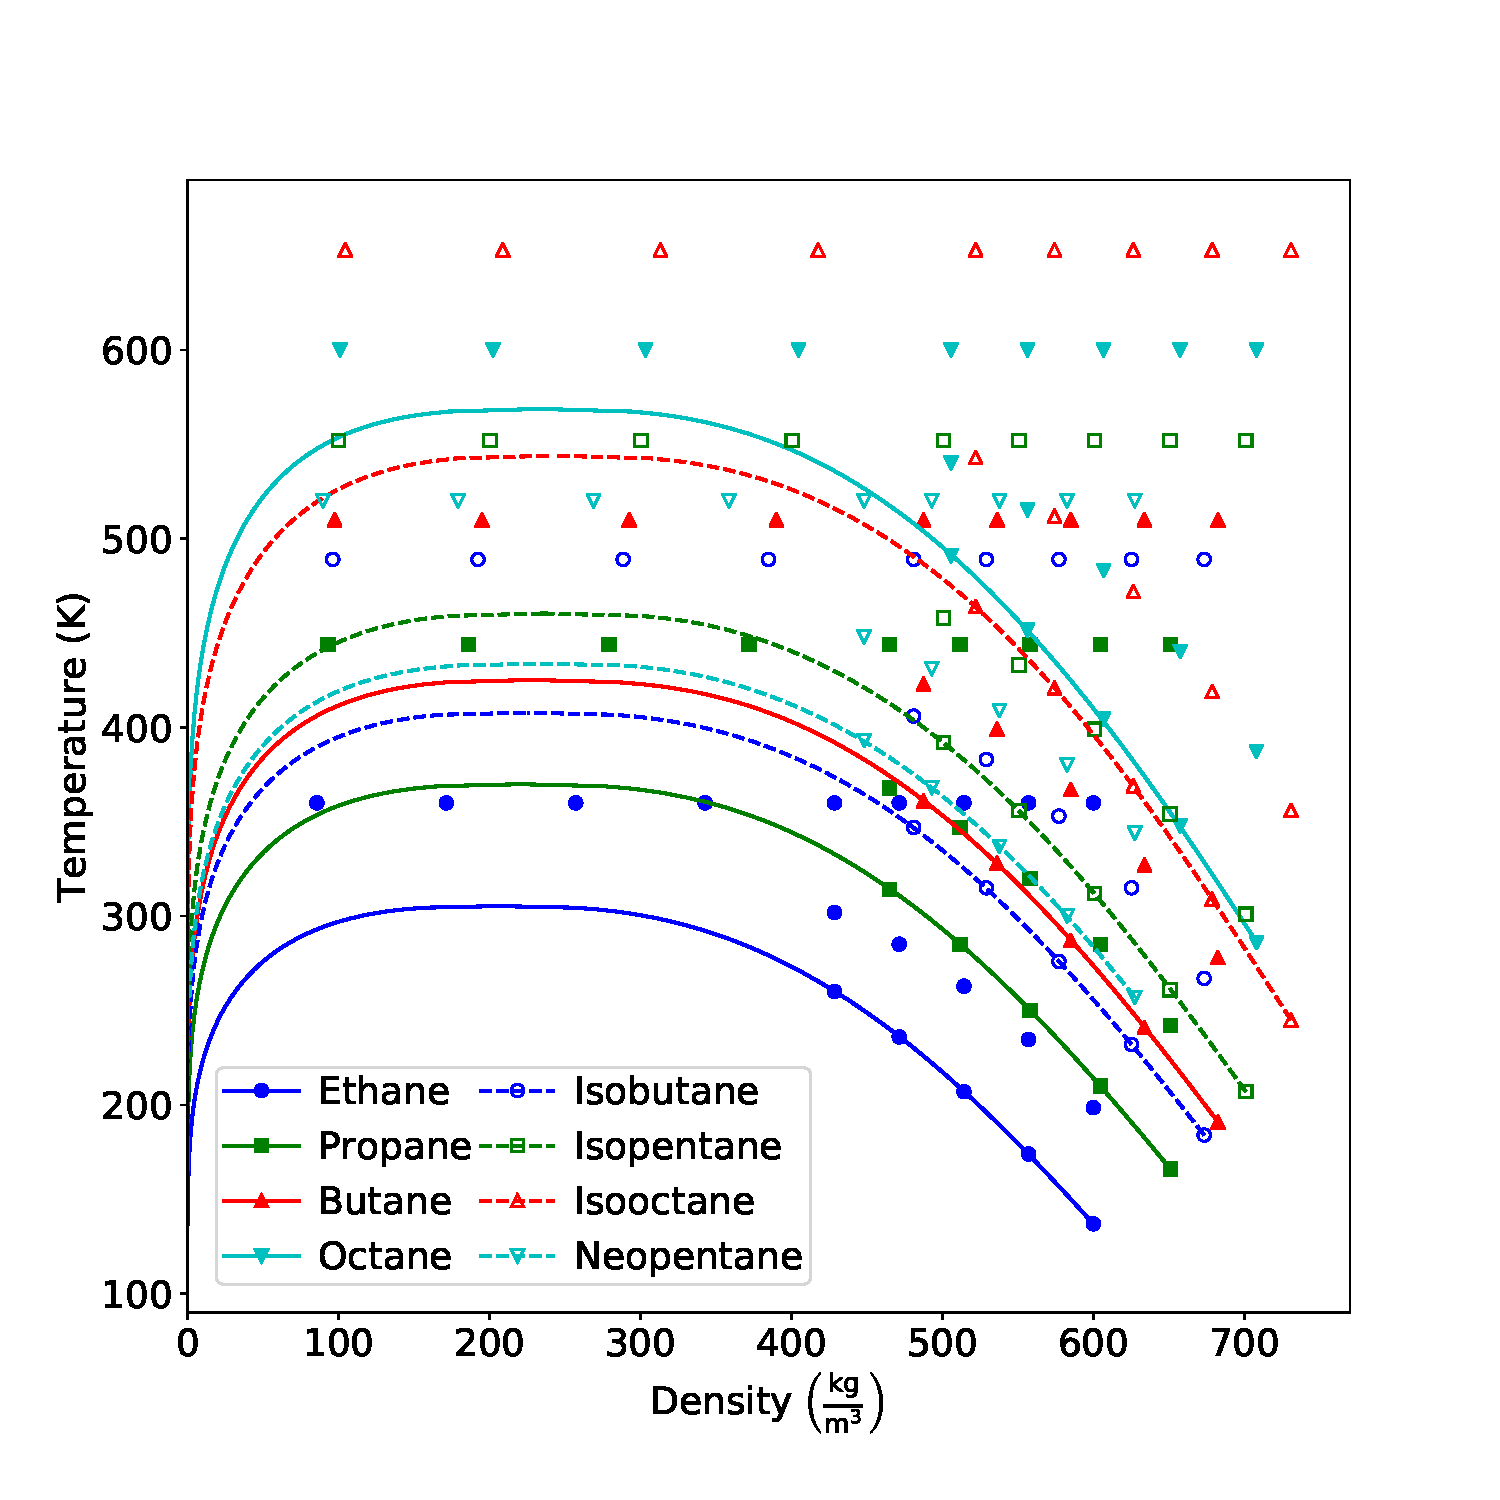
\includegraphics[width=3.2in]{simulation_conditions}
	\caption{State points simulated for each compound studied. A total of 19 simulations are performed: nine densities along the supercritical isotherm and two temperatures along liquid density isochores. Filled symbols and solid lines correspond to \textit{n}-alkanes, while empty symbols and dashed lines correspond to branched alkanes. The REFPROP saturation curve for each compound is included as a reference.}
	\label{fig:simulation_conditions}
\end{figure}

We use isothermal isochoric integration (ITIC) to convert the departure internal energies $(U^{\rm dep})$ and compressibility factors $(Z)$ obtained at the 19 state points to saturated VLE properties, namely, $\rho_{\rm l}^{\rm sat}$ and $P_{\rm v}^{\rm sat}$ \cite{Mostafa_Diss,Postdoc_1}.
The 
%fundamental 
equations for ITIC are: 
\begin{equation} \label{ITIC A}
\frac{A^{\rm dep}}{R_{\rm g}T^{\rm sat}} = \int_{0}^{\rho_{\rm l}^{\rm sat}}\frac{Z-1}{\rho} \partial \rho |_{T = T^{\rm IT}} + \int_{T^{\rm IT}}^{T^{\rm sat}}U^{\rm dep}\partial\left(\frac{1}{R_{\rm g}T}\right)|_{\rho=\rho_{\rm l}^{\rm sat}}
\end{equation}
\begin{equation} \label{ITIC rhov}
\rho_{\rm v}^{\rm sat} \approx \rho_{\rm l}^{\rm sat} \exp \left( \frac{A^{\rm dep}}{R_{\rm g}T^{\rm sat}} + Z_{\rm l}^{\rm sat} - 1 - 2 B_2 \rho_{\rm v}^{\rm sat} - 1.5 B_3 (\rho_{\rm v}^{\rm sat})^2 \right)
\end{equation}
\begin{equation} \label{ITIC Pv}
P_{\rm v}^{\rm sat} \approx \left(1 + B_2 \rho_{\rm v}^{\rm sat} + B_3 (\rho_{\rm v}^{\rm sat})^2\right)\rho_{\rm v}^{\rm sat} R_{\rm g}T^{\rm sat}
\end{equation}
\begin{equation} \label{ITIC Zl}
Z_{\rm l}^{\rm sat} = \frac{P_{\rm v}^{\rm sat}}{\rho_{\rm l}^{\rm sat} R_{\rm g} T^{\rm sat}}
\end{equation}
where $A^{\rm dep} \equiv A-A^{\rm ig}$ is the Helmholtz free energy departure from ideal gas for temperature $(T)$ equal to the saturation temperature $(T^{\rm sat})$ and density $(\rho)$ equal to the saturated liquid density $(\rho_{\rm l}^{\rm sat})$, $U^{\rm dep} \equiv U-U^{\rm ig}$ is the internal energy departure, $Z_{\rm l}^{\rm sat}$ is the saturated liquid compressibility factor $(Z)$, $B_2$ is the second virial coefficient, $B_3$ is the third virial coefficient, $T^{\rm IT}$ is the isothermal temperature, and $R_{\rm g}$ is the universal gas constant. As discussed and validated in our previous work \cite{Postdoc_1}, the $B_2$ and $B_3$ values found in Equations \ref{ITIC rhov}-\ref{ITIC Pv} are calculated using REFPROP correlations \cite{LEMMON-RP91}. Details for this methodology are found in our previous work \cite{Postdoc_1}.  

%\begin{enumerate}
%	\item The compounds simulated in this study are ethane, propane, \textit{n}-butane, \textit{n}-octane, isobutane, isopentane, isohexane, isooctane, and neopentane
%	\item These compounds were selected as a sample set for 2,2,4-trimethylhexane, the compound studied in the 10th Industrial Fluid Properties Simulation Challenge
%	\item We perform NVT simulations in GROMACS along a supercritical isotherm and five isochores that correspond to saturated liquid densities
%	\item We use ITIC to convert the Udep and Z values obtained from the NVT simulations to rholsat and Pvsat
%	\item The specific state points are depicted in Figure, tabulated values are provided in supporting information
%%MRS: probably should give main settings in the text. 
%	\item The GROMACS settings are provided in supporting information
%\end{enumerate}

\subsection{Force field} \label{Force Field}

A united-atom (UA) or anisotropic-united-atom (AUA) representation is used for each compound studied. The UA and AUA groups required for normal and branched alkanes are sp$^3$ hybridized CH$_3$, CH$_2$, CH, and C sites. For most literature models, a single (transferable) parameter set is assigned for each interaction site. However, two exceptions exist for the force fields studied. First, TAMie implements a different set of CH$_3$ parameters for ethane and other alkanes. Second, Potoff reports a ``generalized'' and ``short/long'' CH and C parameter set. The Potoff ``generalized'' parameter set is an attempt at a completely transferable set. However, since the ``generalized'' parameters performed poorly for some compounds, the ``short/long'' parameter set was proposed, where the ``short'' and ``long'' parameters are implemented when the number of carbons in the backbone is $\le 4$ and $> 4$, respectively. 

A fixed bond-length is used for each bond between UA or AUA sites. Although TAMie is an AUA force field, only the terminal CH$_3$ sites have a displacement in the interaction site. This convention is much simpler to implement than other AUA approaches (such as AUA4) where non-terminal (i.e. CH$_2$ and CH) interaction sites also have a displacement distance. For this reason, we do not attempt to simulate the AUA4 force field for any compounds containing CH$_2$ and CH interaction sites. Therefore, the anisotropic shift in a terminal interaction site (i.e. CH$_3$) is treated simply as a longer effective bond-length (see Table \ref{tab:bond-lengths}). The bond-length for all non-terminal sites is 0.154 nm, except for the Errington Exp-6 force field which uses 0.1535 nm for CH$_2$-CH$_2$ bonds.

\begin{table}[h!]
	\caption{Effective bond-lengths (nm) for terminal (CH$_3$) UA or AUA interaction sites. ``Not-applicable'' (``N/A'') signifies that the force field either does not include these site types (e.g. Exp-6 and TraPPE-2) or that a more complicated notation than a simple effective bond-length is required to adequately represent the force field (i.e. AUA4).} \label{tab:bond-lengths}
	\begin{center}
		\begin{tabular}{|c|c|c|c|c|c|}
			\hline
			Bond & TraPPE, Potoff & TAMie & Exp-6 & AUA4 & TraPPE-2 \\ \hline
			CH$_3$-CH$_3$ & 0.154 & 0.194 & 0.1839 & 0.1967 & 0.230 \\ 
			CH$_3$-CH$_2$ & 0.154 & 0.174 & 0.1687 & N/A & N/A \\ 
			CH$_3$-CH & 0.154 & 0.174 & N/A & N/A & N/A \\
			CH$_3$-C & 0.154 & 0.174 & N/A & 0.1751 & N/A \\
			\hline
		\end{tabular}
	\end{center} 
\end{table}

The angle and dihedral energies are computed using the same functional forms and parameters for each force field. Angular bending interactions are evaluated using a harmonic potential:
\begin{equation*}
u^{\rm bend} = \frac{k_\theta}{2} \left(\theta-\theta_0\right)^2
\end{equation*}
where $\theta$ is the instantaneous bond angle, $\theta_0$ is the equilibrium bond angle, and $k_\theta$ is the harmonic force constant which is equal to 62500 K/rad$^2$ for all potentials. Dihedral torsional interactions are determined using a cosine series:
\begin{equation*}
u^{\rm tors} = c_1 [1+\cos{\phi}] + c_2 [1-\cos{2\phi}] + c_3 [1+\cos{3\phi}]
\end{equation*}
where $\phi$ is the dihedral angle and $c_i$ are the Fourier constants. The equilibrium bond angles and torsional parameters are found in Tables \ref{tab:angles}-\ref{tab:torsions}, respectively. 

\begin{table}[h!]
	\caption{Equilibrium bond angles $(\theta_0)$. $x$ and $y$ are values between 0-3.} \label{tab:angles}
	\begin{center}
		\begin{tabular}{|c|c|}
			\hline
			Bending sites & $\theta_0$ (degrees) \\ \hline
			CH$_x$-CH$_2$-CH$_y$ & 114.0 \\ 
			CH$_x$-CH-CH$_y$ & 112.0 \\ 
			CH$_x$-C-CH$_y$ & 109.5 \\  
			\hline
		\end{tabular}
	\end{center} 
\end{table}

\begin{table}[h!]
	\caption{Fourier constants $(c_i)$ in K. $x$ and $y$ are values between 0-3.} \label{tab:torsions}
	\begin{center}
		\begin{tabular}{|c|c|c|c|c|}
			\hline
			Torsion sites & $c_0$ & $c_1$ & $c_2$ & $c_3$ \\ \hline
			CH$_x$-CH$_2$-CH$_2$-CH$_y$ & 0.0 & 355.03 & -68.19 & 791.32 \\ 
            CH$_x$-CH$_2$-CH-CH$_y$ & -251.06 & 428.73 & -111.85 & 441.27 \\
            CH$_x$-CH$_2$-C-CH$_y$ & 0.0 & 0.0 & 0.0 & 461.29 \\
            CH$_x$-CH-CH-CH$_y$ & -251.06 & 428.73 & -111.85 & 441.27 \\
			\hline
		\end{tabular}
	\end{center} 
\end{table}

Non-bonded interactions between two different molecules and united-atom sites separated by more than three bonds are calculated using either a Lennard-Jones 12-6, Mie $\lambda$-6, or Buckingham Exponential-6 potential. The Mie $\lambda$-6 potential is:
\begin{equation} \label{eq:Mie}
u^{\rm vdw}(\epsilon,\sigma,\lambda;r) = \left(\frac{\lambda}{\lambda - 6}\right)\left(\frac{\lambda}{6}\right)^{\frac{6}{\lambda - 6}} \epsilon \left[\left(\frac{\sigma}{r}\right)^\lambda - \left(\frac{\sigma}{r}\right)^6\right]
\end{equation} 
where $u^{\rm vdw}$ is the van der Waals interaction, $\sigma$ is the distance $(r)$ where $u^{\rm vdw} = 0$, $-\epsilon$ is the energy of the potential at the minimum $\left(\text{i.e. }u^{\rm vdw} = -\epsilon \text{ and } \frac{\partial u^{\rm vdw}}{\partial r} = 0 \text{ for } r=r_{\rm min} \right)$, and $\lambda$ is the repulsive exponent. 

Note that the Mie $\lambda$-6 potential reduces to the LJ 12-6 potential for $\lambda = 12$. Therefore, the LJ 12-6 potential can be considered a special subclass of the Mie $\lambda$-6 potential. It is important to mention that, although an attractive exponent of 6 has a strong theoretical basis, $\lambda = 12$ is a historical artifact that was chosen primarily for computational purposes \cite{Allen1987}. For the same reason (i.e. computational efficiency), a common practice to date is to use integer values of $\lambda$ in Equation \ref{eq:Mie}. The non-bonded force field parameters for TraPPE (and TraPPE-2), Potoff, AUA4, and TAMie are provided in Table \ref{tab:nonbonded params}.

\begin{table}[h!]
	\caption{Non-bonded (intermolecular) parameters for TraPPE \cite{TraPPE,Martin1999} (and TraPPE-2 \cite{TraPPEUA2}), Potoff \cite{Mie,Potoff_branched}, AUA4 \cite{AUA4,Nieto2008}, and TAMie \cite{TAMie,Weidler2016} force fields. The ``short/long'' Potoff CH and C parameters are included in parenthesis. The ethane specific parameters for TAMie are included in parenthesis.} \label{tab:nonbonded params}
	\begin{center}
		\begin{tabular}{|c|c|c|c|c|c|c|}
			\hline
			\multicolumn{1}{|c}{} & \multicolumn{3}{|c}{TraPPE  (TraPPE-2 )} & \multicolumn{3}{|c|}{Potoff (S/L)}  \\ \hline
			United-atom & $\epsilon$ (K) & $\sigma$ (nm) & $\lambda$ & $\epsilon$ (K) & $\sigma$ (nm) & $\lambda$ \\ \hline
			CH$_3$ & 98 (134.5)  & 0.375 (0.352) & 12 & 121.25 & 0.3783 & 16  \\ 
			CH$_2$ & 46 & 0.395 & 12 & 61 & 0.399 & 16 \\ 
			CH & 10 & 0.468 & 12 & 15 (15/14) & 0.46 (0.47/0.47) & 16\\
			C & 0.5 & 0.640 & 12 & 1.2 (1.45/1.2) & 0.61 (0.61/0.62) & 16\\
			\hline
			\multicolumn{1}{|c}{} & \multicolumn{3}{|c}{AUA4} & \multicolumn{3}{|c|}{TAMie} \\ \hline
			CH$_3$ & 120.15  & 0.3607 & 12 & 136.318 (130.780) & 0.36034 (0.36463) & 14 \\ 
			CH$_2$ & 86.29 & 0.3461 & 12 & 52.9133 & 0.40400 & 14 \\ 
			CH & 50.98 & 0.3363 & 12 & 14.5392 & 0.43656 & 14\\
			C & 15.04 & 0.244 & 12 & N/A & N/A & N/A\\
			\hline
		\end{tabular}
	\end{center} 
\end{table}

%\begin{table}[h!]
%	\caption{Non-bonded (intermolecular) parameters for TraPPE-UA, Potoff, and TAMie force fields. The ``short/long'' Potoff CH and C parameters are included in parenthesis. The ethane specific parameters for TAMie are included in parenthesis.} \label{tab:nonbonded params}
%	\begin{center}
%		\begin{tabular}{|c|c|c|c|c|c|c|c|c|c|}
%			\hline
%			\multicolumn{1}{|c}{} & \multicolumn{3}{|c}{TraPPE-UA} & \multicolumn{3}{|c}{Potoff} & \multicolumn{3}{|c|}{TAMie} \\ \hline
%			United-atom & $\epsilon$ (K) & $\sigma$ (nm) & $\lambda$ & $\epsilon$ (K) & $\sigma$ (nm) & $\lambda$ & $\epsilon$ (K) & $\sigma$ (nm) & $\lambda$ \\ \hline
%			CH$_3$ & 98 & 0.375 & 12 & 121.25 & 0.3783 & 16 & 136.318 (130.780) & 0.36034 (0.36463) & 14 \\ 
%			CH$_2$ & 46 & 0.395 & 12 & 61 & 0.399 & 16 & 52.9133 & 0.40400 & 14\\ 
%			CH & 10 & 0.468 & 12 & 15 (15/14) & 0.46 (0.47/0.47) & 16 & 14.5392 & 0.43656 & 14 \\
%			C & 0.5 & 0.640 & 12 & 1.2 (1.45/1.2) & 0.61 (0.61/0.62) & 16 & N/A & N/A & N/A \\
%			\hline
%		\end{tabular}
%	\end{center} 
%\end{table}
%
%\begin{table}[h!]
%	\caption{Non-bonded (intermolecular) parameters for TraPPE, Potoff, and TAMie force fields. The TraPPE-2 parameters for CH$_3$ are included in parenthesis. The ``short/long'' Potoff CH and C parameters are included in parenthesis. The ethane specific parameters for TAMie are included in parenthesis.} \label{tab:nonbonded params}
%	\begin{center}
%		\begin{tabular}{|c|c|c|c|c|c|c|c|c|c|}
%			\hline
%			\multicolumn{1}{|c}{} & \multicolumn{2}{|c}{TraPPE LJ 12-6} & \multicolumn{2}{|c}{Potoff Mie 16-6} & \multicolumn{2}{|c|}{TAMie Mie 14-6} \\ \hline
%			United-atom & $\epsilon$ (K) & $\sigma$ (nm) & $\epsilon$ (K) & $\sigma$ (nm) & $\epsilon$ (K) & $\sigma$ (nm) \\ \hline
%			CH$_3$ & 98 (134.5)  & 0.375 (0.352) & 121.25 & 0.3783 & 136.318 (130.780) & 0.36034 (0.36463) \\ 
%			CH$_2$ & 46 & 0.395 & 61 & 0.399 & 52.9133 & 0.40400 \\ 
%			CH & 10 & 0.468 & 15 (15/14) & 0.46 (0.47/0.47)  & 14.5392 & 0.43656  \\
%			C & 0.5 & 0.640 & 1.2 (1.45/1.2) & 0.61 (0.61/0.62)& N/A & N/A  \\
%			\hline
%		\end{tabular}
%	\end{center} 
%\end{table}
%
%\begin{table}[h!]
%	\caption{Non-bonded (intermolecular) parameters for TraPPE-2 and AUA4. Only the , Potoff, and TAMie force fields. The ``short/long'' Potoff CH and C parameters are included in parenthesis.} \label{tab:nonbonded params2}
%	\begin{center}
%		\begin{tabular}{|c|c|c|c|c|c|c|}
%			\hline
%			\multicolumn{1}{|c}{} & \multicolumn{3}{|c}{TraPPE-UA} & \multicolumn{3}{|c|}{Potoff} \\ \hline
%			United-atom & $\epsilon$ (K) & $\sigma$ (nm) & $\lambda$ & $\epsilon$ (K) & $\sigma$ (nm) & $\lambda$ \\ \hline
%			CH$_3$ & 98 & 0.375 & 12 & 121.25 & 0.3783 & 16  \\ 
%			CH$_2$ & 46 & 0.395 & 12 & 61 & 0.399 & 16 \\ 
%			CH & 10 & 0.468 & 12 & 15 (15/14) & 0.46 (0.47/0.47) & 16 \\
%			C & 0.5 & 0.640 & 12 & 1.2 (1.45/1.2) & 0.61 (0.61/0.62) & 16 \\
%			\hline
%		\end{tabular}
%	\end{center} 
%\end{table}

Non-bonded interactions between two different site types (i.e. cross-interactions) are determined using Lorentz-Berthelot combining rules \cite{Allen1987} for $\epsilon$ and $\sigma$ with an arithmetic mean for the repulsive exponent $(\lambda)$ (as recommended by Potoff and Bernard-Brunel \cite{Mie}):
\begin{equation} \label{eq:Lorentz-Berthelot_eps}
\epsilon_{ij} = \sqrt{\epsilon_{ii} \epsilon_{jj}}
\end{equation}
\begin{equation} \label{eq:Lorentz-Berthelot_sig}
\sigma_{ij} = \frac{\sigma_{ii} + \sigma_{jj}}{2}
\end{equation}
\begin{equation} \label{eq:Lorentz-Berthelot_lam}
\lambda_{ij} = \frac{\lambda_{ii} + \lambda_{jj}}{2}
\end{equation}
where the $ij$ subscript refers to cross-interactions and the subscripts $ii$ and $jj$ refer to same-site interactions. 

%\begin{enumerate}
%	\item For each compound studied, we use a united-atom representation as defined by the TraPPE (and Mie) force fields. For normal and branched alkanes this consists of CH3, CH2, CH, and C sites.
%	\item We use fixed bond-lengths, harmonic angles, cosine series for torsions, and exclude 1-4 nonbonded interactions 
%	\item Bonded parameters are provided in supporting information
%	\item Nonbonded interactions for intermolecular and intramolecular sites separated by more than 3 bonds are represented using a Mie potential, which can be viewed as a generalized Lennard-Jones
%%MRS: need to make it clearer what your hypothesis is, then.  If it's just ``Mie not good'', then restrict it.  If the goal is to find something better, which might be more impactful. But it can be a short paper. If its ``nothing existing is good'', then will need to include others.
%%MRS: Looking more carefully, I think your main idea is not that Mie isn't that good, but NONE of the existing UA isotropic functional forms are not that good. That is a more general conclusion, but doesn't force you to posit a new one within the scope of this paper. It does make a stronger statement; if you say ``Mie isn't good'', then people will wonder, why don't you just say what is good.  If you say none of the ``standard UA approaches are good'' that's more important.   You MIGHT need to say ``But this approach can work''.  That might require more work than there is time for this time.
%	\item (Maybe include Exp-6 and extended Lennard-Jones, i.e. 12-10-8-6)
%%MRS: when you say ``rigorous bayesian'', you should be more specific what analysis doing.
%%MRS: My instinct, if ``anisotropic'' UA works for this system, it might not be worth it that much to develop a new functional form.  Unless there's strong reason it might be useful more generally.  we can discuss goals a bit; it really depends on goals. 
%\end{enumerate}

\section{Case study for alkanes} \label{Case Study}

The purpose of this case study is to demonstrate that the existing UA and AUA force fields for normal and branched alkanes that were parameterized with VLE properties do not predict the proper $PVT$ behavior at higher temperatures and pressures (with the exception of ethane for the TraPPE-2 potential). Figures \ref{fig:IC_normal_alkanes} and \ref{fig:IC_branched_alkanes} plot the compressibility factor with respect to inverse temperature for \textit{n}-alkanes and branched alkanes, respectively. Note that saturation corresponds to $Z \approx 0$ for each isochore. 

The ``Potoff'' results in Figure \ref{fig:IC_branched_alkanes} are only for the the ``short/long'' model, since the ``short/long'' model is more accurate than the ``generalized'' model. The results for the ``generalized'' model do not provide any additional insight but are found in the Supporting Information. 

%Several force fields in the literature have been optimized to agree with VLE properties for normal and branched alkanes. Two of the most widely used united-atom based force fields are the TraPPE LJ 12-6 and Potoff Mie 16-6.

%It has been demonstrated that the united-atom LJ 12-6 potential cannot adequately estimate both $\rho_{\rm l}^{\rm sat}$ and $P_{\rm v}^{\rm sat}$. By contrast, when properly optimized, the Mie 16-6 potential can accurately predict both $\rho_{\rm l}^{\rm sat}$ and $P_{\rm v}^{\rm sat}$ over a wide temperature range. However, there is some concern that increasing the repulsive exponent (in this case, from 12 to 16) might have some undesirable consequences, especially at high pressures, where close range interactions will become more significant.

Figure \ref{fig:IC_normal_alkanes} demonstrates that the existing literature force fields for \textit{n}-alkanes, while accurate for VLE, do not capture the correct $PVT$ behavior at high pressures, i.e. the  higher temperatures and highest isochore densities $(\rho_0$ and $\rho_1)$. Figure \ref{fig:IC_branched_alkanes} shows that these force fields are typically less reliable at VLE for branched alkanes than for \textit{n}-alkanes but, more importantly, the same erroneous trend in $Z$ is observed as in Figure \ref{fig:IC_normal_alkanes}.  

The one exception is the TraPPE-2 model for ethane, which reproduces the entire $PVT$ phase space simulated. This result is somewhat surprising considering the TraPPE-2 model has only three fitting parameters ($\epsilon$, $\sigma$, and the effective bond-length) while the TAMie model has an additional fitting parameter $(\lambda)$. It is important to note that TraPPE-2 uses a much longer effective bond-length of 0.230 nm while TAMie did not consider bond-lengths larger than 0.194 nm (see Table \ref{tab:bond-lengths}). Therefore, the fact that the TraPPE-2 force field extrapolates to high pressures better than TAMie suggests that, at high pressures, it is important to account for hydrogens either explicitly (AA model) or with a longer effective bond-length than that typically used for AUA models. It is also possible that a four parameter optimization, such as that used by TAMie, is over fit to the VLE data and would perform better if high pressure $PVT$ data were included in the parameterization.

\begin{figure}[htb!]
	\centering
	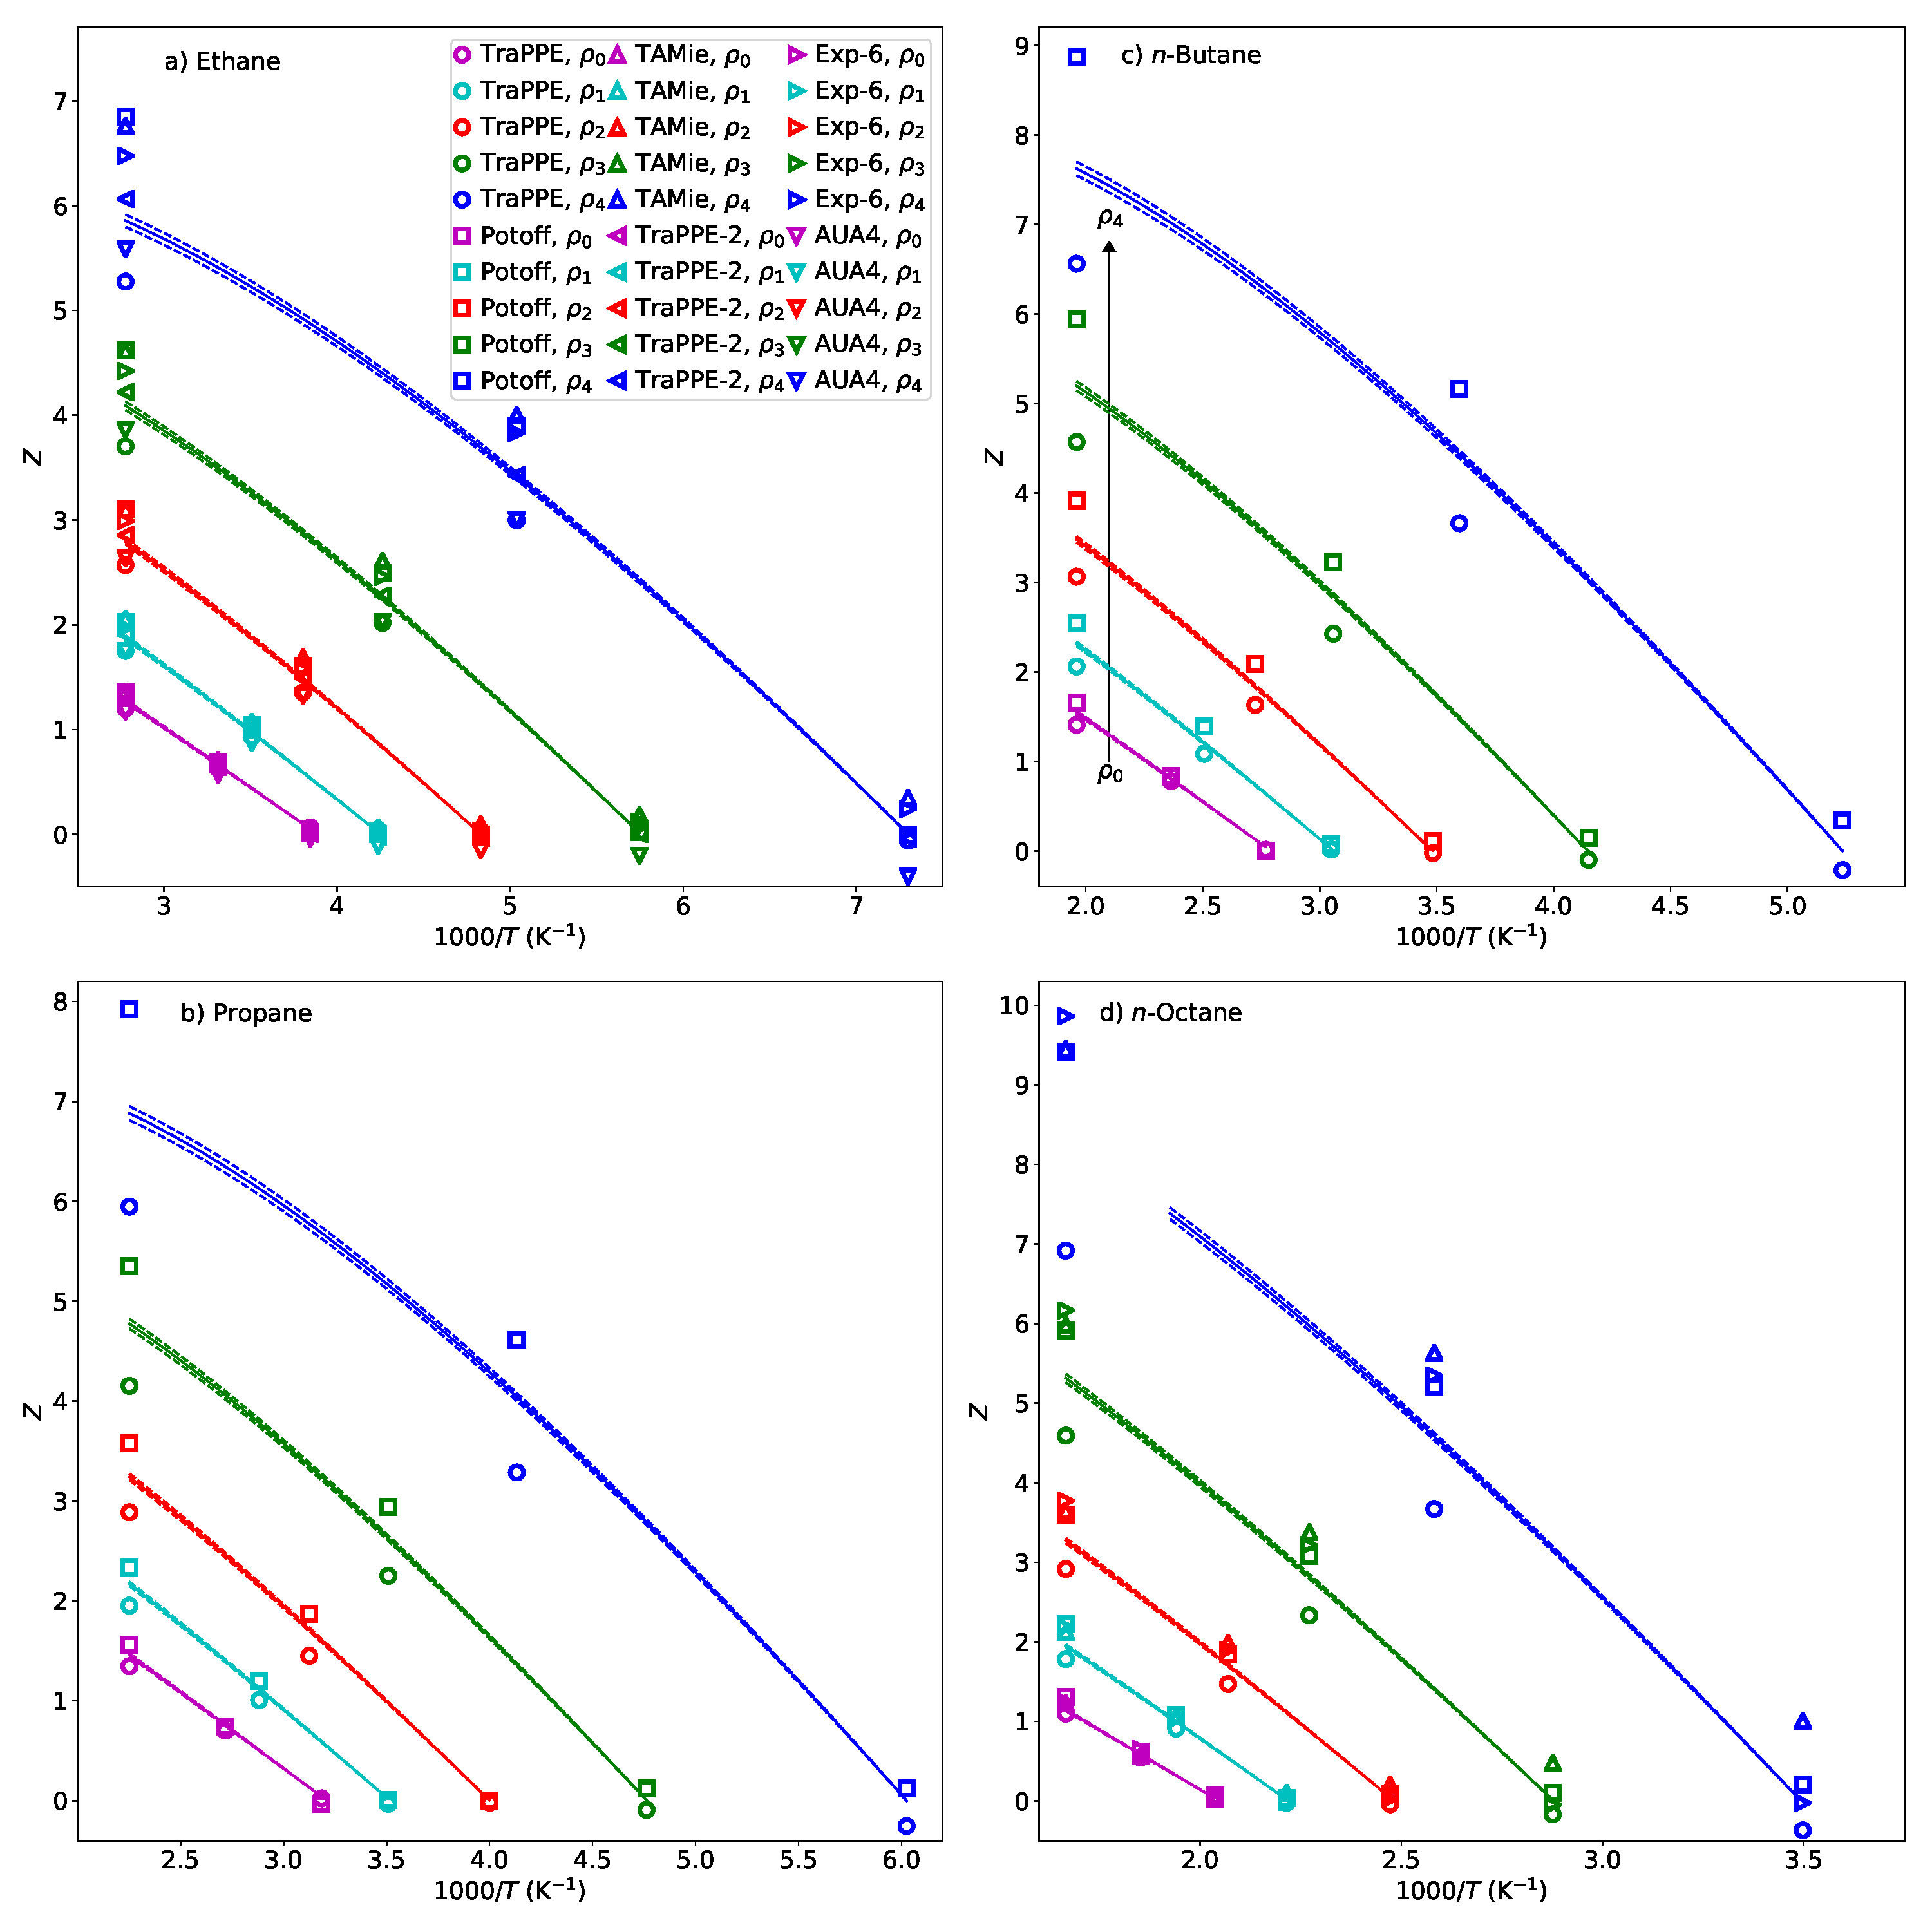
\includegraphics[width=6.4in]{IC_normal_alkanes_all_models}
	\caption{Compressibility factors $(Z)$ along isochores agree at saturation $(Z \approx 0)$ but deviate strongly at higher pressures. Densities are distinguished by color, increase vertically, and are labeled such that $\rho_0 > \rho_1 > \rho_2 > \rho_3 > \rho_4$.  Panels a)-d) correspond to ethane, propane, \textit{n}-butane, and \textit{n}-octane, respectively. TraPPE and Potoff simulation results are depicted using open circles and squares, respectively, with error bars representing two times the standard deviation of the fluctuations from a single simulation. Solid lines represent REFPROP correlations, with dashed lines representing a 1\% uncertainty in REFPROP values. Simulation error bars are approximately one symbol size.}
	\label{fig:IC_normal_alkanes}
\end{figure}

\begin{figure}[htb!]
	\centering
	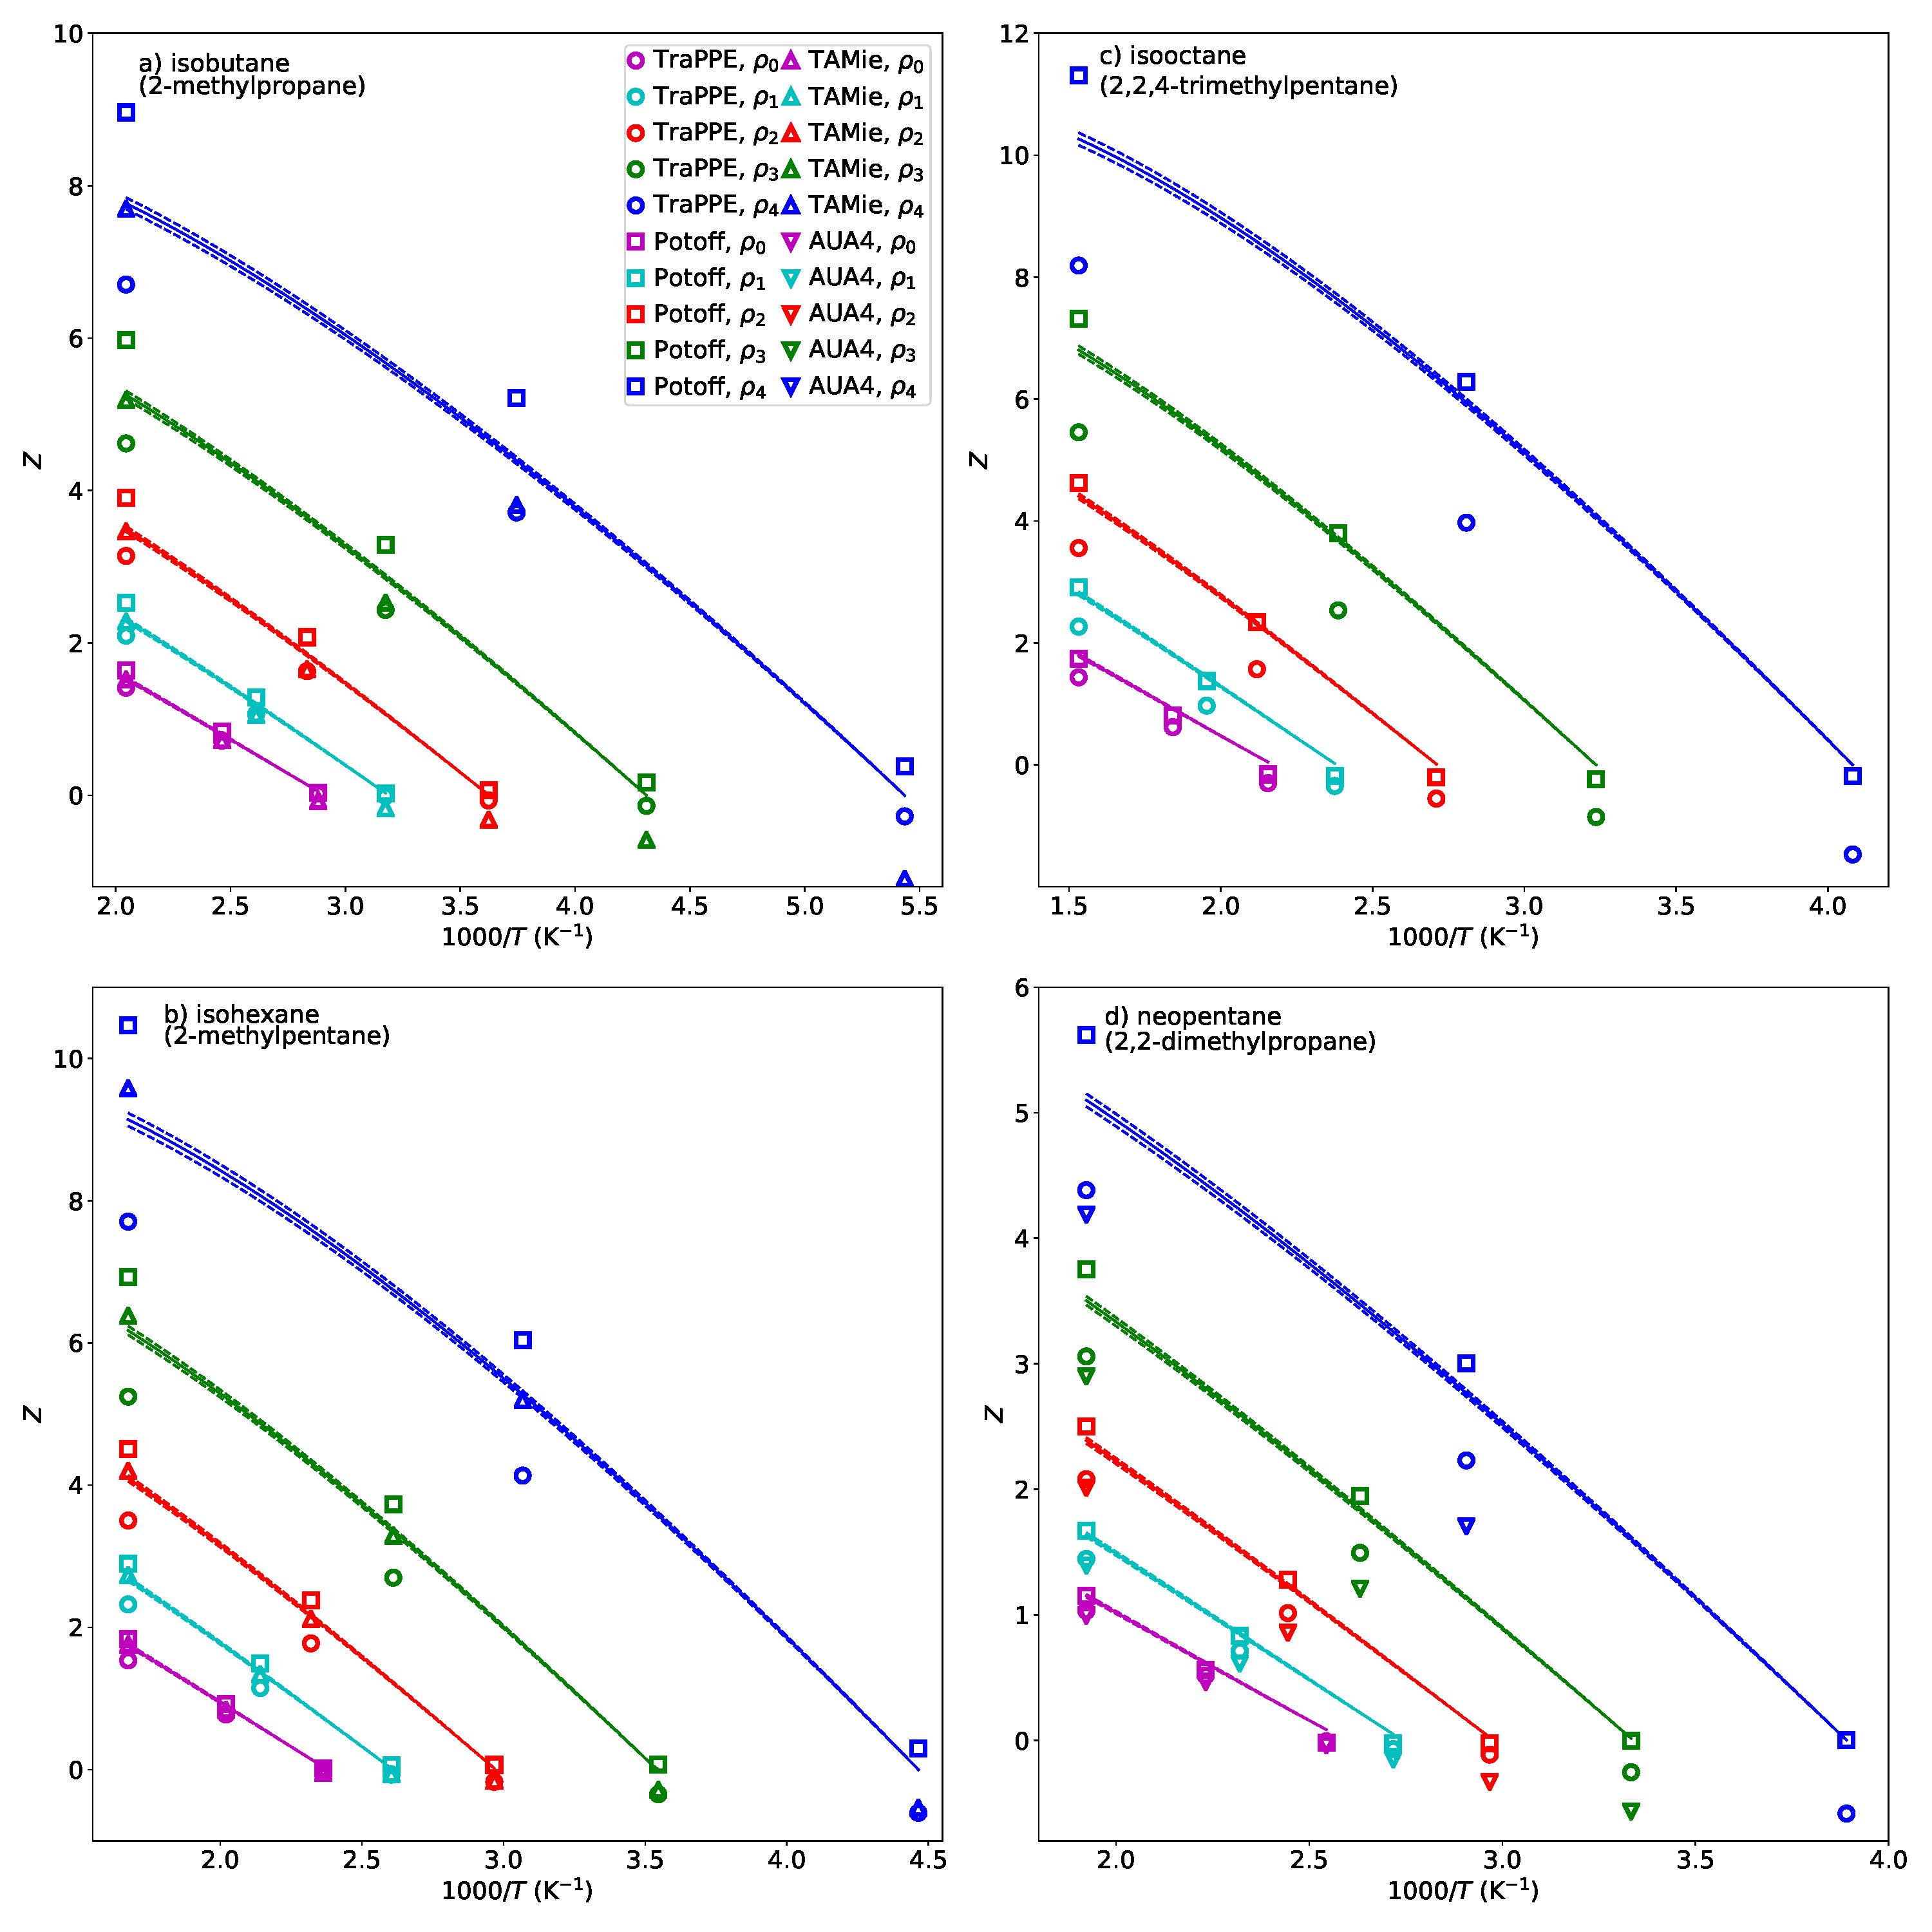
\includegraphics[width=6.4in]{IC_branched_alkanes_all_models}
	\caption{Compressibility factors $(Z)$ along isochores for branched alkanes are not as accurate as normal alkanes at saturation $(Z \approx 0)$ and deviate strongly at higher pressures. Panels a)-d) correspond to isobutane, isopentane, isooctane, and neopentane, respectively. Symbols, lines, uncertainties, and formatting are the same as those in Figure \ref{fig:IC_normal_alkanes}.}
	\label{fig:IC_branched_alkanes}
\end{figure}

% I am going to change isopentane to isohexane so that it uses Potoff 'long', to have a better representation of compounds.

In general, a clear bias is observed for the LJ 12-6 potentials (TraPPE-UA and AUA4) and the Mie $\lambda$-6 potentials (Potoff and TAMie). Specifically, the LJ 12-6 and Mie $\lambda$-6 potentials under- and over-predict $Z$ at high pressures, respectively. These results are intuitive as the repulsive barriers are steeper for the respective Mie 16-6 and 14-6 potentials of the Potoff and TAMie force fields. Another surprising trend is that the Errington (AUA Exp-6) model also has a positive bias at high pressures, suggesting that an exponential repulsive barrier is also too steep. Unfortunately, a direct comparison of the non-bonded potentials for AUA models is difficult because each model has a different anisotropic displacement. By contrast, a comparison of TraPPE-UA and Potoff is straightforward because they use the same bond-lengths and the same non-bonded potential (Equation \ref{eq:Mie}). For this reason, the remainder of this document focuses on the united-atom Mie $\lambda$-6 potentials where all bond-lengths are 0.154 nm.

Since the TraPPE-UA (LJ 12-6) potential under-predicts $Z$ and the Potoff (UA Mie 16-6) potential over-predicts $Z$, it seems reasonable that a UA Mie 13-6, 14-6, or 15-6 model would demonstrate the proper trend, if parameterized appropriately. However, as demonstrated in Section \ref{Results}, there does not exist a set of $\epsilon$, $\sigma$, and $\lambda$ that reasonably predicts $\rho_{\rm l}^{\rm sat}$, $P_{\rm v}^{\rm sat}$, and $PVT$ of supercritical fluids and compressed liquids for the UA model. To understand this point, it is important to remember that the UA LJ 12-6 (TraPPE-UA) force field cannot adequately predict both $\rho_{\rm l}^{\rm sat}$ and $P_{\rm v}^{\rm sat}$. In other words, determining the optimal value of $\lambda$ for predicting $PVT$ of supercritical fluids and compressed liquids does not guarantee accurate prediction of $P_{\rm v}^{\rm sat}$. See Section \ref{Results} for a further discussion.

%Although the TAMie potential uses a softer repulsive exponent than Potoff (14 instead of 16), it consistently over-predicts the pressure for supercritical fluids and compressed liquids. The same is true for the Errington Exp-6 model. By contrast, the TraPPE-2 potential provides extremely reliable estimates of $\rho_{\rm l}^{\rm sat}$, $P_{\rm v}^{\rm sat}$, and the PVT behavior at high pressures and temperatures. Although the TraPPE-2 model is only available for ethane and ethylene, these results suggest that at extreme pressures either an AUA or AA model should be used to better account for the hydrogens. That being said, alternative functional forms, such as the extended Lennard-Jones, should also be considered.

% although the 12-6 potential is too soft and the 16-6 potential is too hard, the optimal exponent i

%\begin{enumerate}
%	\item Several force fields in the literature have been optimized to agree with VLE properties (TraPPE, Potoff, TraPPE-2, TAMie, Errington, AUA4)
%	\item TraPPE, Potoff, and AUA4 have parameters for each compound studied, while TraPPE-2 only has parameters for ethane, TAMie has parameters for all except isooctane and neopentane (containing a C group), and ErrExp-6 only has parameters for the \textit{n}-alkanes
%%MRS: for figures: be more explicit about what point the data in the figures are supposed to support.
%	\item Figure: Z vs 1000/T for ethane, propane, n-butane, and n-octane
%	\item Figure: Z vs 1000/T for isobutane, isopropane, isohexane, isooctane and neopentane 
%	\item PVT (Z) trends are inaccurate for both TraPPE and Potoff at high pressures, i.e. non-VLE conditions. Specifically, the TraPPE 12-6 under-predicts while 16-6 over-predicts
%	\item Although these results might suggest that a 14-6 potential would work best, recall that the TraPPE 12-6 does not accurately predict Pvsat. 
%	\item Since TraPPE and Potoff use slightly different objective functions we want to perform an equivalent analysis for different values of lambda
%	\item Hypothesis that we want to test is that there does not exist a set of epsilon, sigma, and lambda that provides reasonable VLE, supercritical fluid, and compressed liquid (for ethane I already know this is not feasible. For n-alkanes I know that the 16-6 cannot accomplish this, but I am not sure about 14-6 or 15-6.)
%	%%% RAM: Do we want to include results for the AUA models in the case study, future work, or supporting information?
%        %%% MRS: it changes the scope a lot.  You have to decide.  ``Not mie'' is simpler, can get out faster.  
%	\item AUA LJ 12-6 is much more accurate for ethane
%	\item AUA Mie 14-6 potential is not much better than UA Mie 16-6 for n-alkanes
%	\item AUA Exp-6 force field is not much better than UA Mie 16-6 for n-alkanes
%	\item No results for AUA4
%\end{enumerate}

\section{Methods II} \label{Methods II}

The results presented in Section \ref{Case Study} demonstrate that none of the existing force fields studied reproduce the $PVT$ behavior for supercritical fluids and compressed liquids. However, recall that each of these force fields was parameterized using only VLE properties. Therefore, it is possible that including both VLE and $PVT$ properties in the parameterization objective function will improve the results. However, if no combination of $\epsilon$, $\sigma$, and $\lambda$ is capable of predicting VLE properties and $PVT$ behavior, we can conclude that the UA Mie $\lambda$-6 potential (and Lennard-Jones 12-6 as a special case) is inadequate for this purpose and, therefore, should not be used when developing FEOS with molecular simulation results.

In order to rigorously quantify if the UA Mie $\lambda$-6 potential is ``adequate'', we perform a Bayesian inference analysis. We refer the reader to the literature for a thorough discussion of Bayesian statistics. In Section \ref{Bayesian Analysis}, we review some basic concepts of Bayes theorem, we define the posterior, likelihood, and prior functions, and we discuss the Markov Chain Monte Carlo (MCMC) sampling approach. As MCMC can be computationally burdensome, especially when coupled with molecular simulations, we use Multistate Bennett Acceptance Ratio (MBAR) as a surrogate model to reduce the computational cost for determining the VLE properties $\rho_{\rm l}^{\rm sat}$ and $P_{\rm v}^{\rm sat}$ and $Z$ of the supercritical fluids and compressed liquids (see Section \ref{Surrogate Model}).

The Bayesian inference analysis for CH$_3$ and CH$_2$ sites is performed sequentially. Specifically, rather than sampling from a four-dimensional (i.e. $\epsilon_{\rm CH_3}, \epsilon_{\rm CH_2}, \sigma_{\rm CH_3}, \sigma_{\rm CH_2}$ for a given value of $\lambda_{\rm CH_3}$ and $\lambda_{\rm CH_2}$) Markov Chain, we implement a sequential two-dimensional approach by assuming the CH$_3$ parameters from ethane are transferable to propane, \textit{n}-butane, and \textit{n}-octane. As mentioned in Section \ref{Force Field}, it is common to limit $\lambda$ to integer values. Although sampling from discrete values is possible with MCMC, because of the strong correlation between $\epsilon$ and $\lambda$ advanced sampling methods are required to achieve good acceptance ratios when varying $\lambda$ by an integer amount. For this reason, we perform the MCMC analysis using fixed values of $\lambda$. This approach is computationally more efficient since we are only concerned with a few values of $\lambda$ (i.e. 12-18). Finally, since the CH$_3$ and CH$_2$ results are similar and suggest that a UA Mie $\lambda$-6 potential cannot estimate both VLE and $PVT$, we did not find it necessary to repeat this process for the CH and C interaction sites.   

%\begin{enumerate}
%	\item We use Bayesian inference with MCMC to quantify the uncertainty in the force field parameters
%	%%%% RAM: Do we even need to perform an MCMC analysis? It is kind of overkill. We could just plot the credible regions by scanning the parameter space.
%        %%%% MRS: agreed.
%	\item We perform direct molecular simulation for several reference force field parameter sets
%	\item We use MBAR-ITIC to predict rholsat and Pvsat with non-simulated force field parameters
%	\item We use MBAR to propagate the parameter uncertainties from VLE to Z of compressed liquids/supercritical
%	\item We perform this analysis for CH3 and CH2 sequentially and independently. 
%%MRS: Not sure this is a Markov Chain? Unless doing MCMC. Would suggest avoiding MCMC for now; we don't know how long it would take.
%In other words, the Markov Chain only samples a 2-dimensional space. % RAM: Andrei and I feel like doing this for CH and C is more work than necessary
%%MRS: not sure what you are saying here. Seems like you do need to do some optimization with C and CH if you are making blanket claims about whether Mie (or other potentials) work or not.  I guess you could justify by saying that if CH2 and CH3 don't work for normal alkanes, no point in proving it for branched alkanes.
%\end{enumerate}

\subsection{Bayesian Analysis} \label{Bayesian Analysis}

Bayesian inference is used to quantify the uncertainty in the non-bonded parameters $(\epsilon$ and $\sigma)$ and to determine the evidence for different values of $\lambda$. 
Bayes theorem states that
\begin{equation} \label{Bayes Theorem}
Pr(\theta|D) = \frac{Pr(D|\theta)Pr(\theta)}{Pr(D)}
\end{equation}
where $Pr$ denotes a probability distribution function, $\theta$ is the parameter set (i.e. $\epsilon$ and $\sigma$ for a given Mie $\lambda$-6 potential), and $D$ are the data. $Pr(\theta|D)$ is commonly referred to as the ``posterior, $Pr(D|\theta)$ is the ``likelihood'' (alternatively expressed as $L(\theta|D)$), $Pr(\theta)$ is the ``prior'', and $Pr(D)$ is a normalization constant. The evidence for different values of $\lambda$ is determined by integrating the numerator of Equation \ref{Bayes Theorem} for all values of $\epsilon$ and $\sigma$. Note that this can be viewed as marginalizing the three-dimensional distribution with respect to $\lambda$. The Bayes factor for two different values of $\lambda$ is obtained from the ratio of the respective evidences. 

Markov Chain Monte Carlo (MCMC) is the traditional approach for numerically sampling from the probability distribution $Pr(\theta|D)$. A Markov Chain is created by proposing new $\epsilon$ or $\sigma$ values and accepting those moves based on the ratio of the probability between the previous parameter set and the proposed parameter set:
\begin{equation} \label{eq:Acceptance}
\alpha = \min\left(1,\frac{Pr(\theta_{i+1}|D)}{Pr(\theta_i|D)}\right)
\end{equation} 
where $\alpha$ is the acceptance probability, $\theta_i$ is the previous parameter set, and $\theta_{i+1}$ is the proposed parameter set. The amount to which $\epsilon$ or $\sigma$ is varied $(\delta \epsilon $ and $\delta \sigma)$ for each MCMC step is tuned such that approximately $\frac{1}{3}$ of the moves are accepted. This ``tuning'' period (also referred to as a ``burn-in'' period) is followed by a production period where $\delta \epsilon $ and $\delta \sigma$ do not change. Details for MCMC are provided in Supporting Information (i.e. number of steps for burn-in and production, frequency that step sizes are updated, resulting acceptance percentages, etc.).

Because MCMC moves are accepted based on Equation \ref{eq:Acceptance} and the denominator in Equation \ref{Bayes Theorem} (i.e $(Pr(D)$) does not depend on $\theta$, the acceptance probability is independent of $Pr(D)$. Also, we use a ``non-informative prior'' such that the acceptance probability is independent of $Pr(\theta)$ (although we do include a lower bound that the parameters are positive, i.e. $Pr(\theta)$ is uniform for all values of $\epsilon$, $\sigma$, and $\lambda$ greater than 0). Therefore, the probability of accepting $\theta_{i+1}$ is based completely on the likelihood. For this reason, we discuss in some detail how we calculate $L(\theta|D)$.  

The likelihood is calculated using a multi-variable normal distribution. The variance accounts for the uncertainties of both the experimental data and the computational analysis (i.e. the methods discussed in Section \ref{Surrogate Model}). The uncertainties are assumed to be independent such that the combined variance is the sum of the experimental and computational variances \cite{Bay_MD}.

The parameter sets sampled from MCMC $(\theta_{\rm MCMC})$ provide an estimate of the uncertainty in $\theta$ (i.e. $\epsilon$ and $\sigma$). Figure \ref{fig:MCMC_Mie_14_16_propane_butane_octane} in Section \ref{Results} depicts the uncertainty in the parameters. This parameter uncertainty propagates when estimating another property $(q)$, which may or may not be included in $D$. For example, although $D$ only consists of VLE properties ($\rho_{\rm l}^{\rm sat}$ and $P_{\rm v}^{\rm sat}$, specifically) we also propagate the uncertainties in $\epsilon$ and $\sigma$ to $Z$ at high temperatures and pressures by implementing posterior prediction. The probability distribution of $q$ $(Pr(q|D))$ is often approximated by developing a histogram of $q$ for the MCMC parameter sets, i.e. $q(\theta_{\rm MCMC})$. Since a large number of MCMC samples are required for adequate representations of $Pr(\theta|D)$ and $Pr(q|D)$, MCMC is computationally infeasible when a direct molecular simulation is required for every $\theta_{\rm MCMC}$. For this reason, a surrogate model is used to approximate $L(\theta|D)$ (and, thereby, $Pr(\theta|D)$) and $q(\theta_{\rm MCMC})$ (and, thereby, $Pr(q|D)$).
%Perhaps I should be more specific. The surrogate model is not for estimating L, it is for estimating q (or y if I want to define L in terms of y or yhat)
  
%
%other properties by computing  predicted with that force field. For example, the uncertainties in $\epsilon$ and $\sigma$ are determined using VLE proper In this study, $D$ consists of VLE properties ($\rho_{\rm l}^{\rm sat}$ and $P_{\rm v}^{\rm sat}$, specifically) but the uncertainties in $\epsilon$ and $\sigma$ 

 

% With MCMC it is not necessary to estimate $Pr(D)$ because MC moves are accepted based on the ratio of $Pr(\theta_i|D)$ and $Pr(\theta_{i+1}|D)$

%\begin{enumerate}
%	\item By quantifying the uncertainty in epsilon and sigma for a given lambda, we can determine if the Mie potential is adequate for reproducing VLE and compressed liquid/supercritical pressures
%	\item Posterior includes saturated liquid density and vapor pressure
%	%%% RAM: Or should we compare several different posteriors? I.e. include rholsat and Pvsat, or rholsat and highP, or all three?
%        %%% MRS: which experiments to incldue are a design choice.  You either specify the experiments you require, or you could show which models are valid for predicting which proprerties.  
%	\item Markov Chain Monte Carlo is used to sample % RAM: Again, do we need to do MCMC or can we simplify things by just performing a 2-D scan
%	\item Details for MCMC are provided in supporting information (i.e. number of steps for burn-in and production, frequency that step sizes are updated, resulting acceptance percentages, etc.)
%	\item The parameter uncertainty is propagated when predicting high pressures
%	% RAM:  No longer finding the optimal lambda for high pressures \item To determine the optimal value of lambda for compressed liquid pressures, we redefine the posterior using only saturated liquid density and compressed liquid pressures  
%\end{enumerate}

\subsection{Surrogate Model} \label{Surrogate Model}

A typical Markov Chain requires $O(10^4$-$10^5)$ Monte Carlo steps, where the likelihood function must be evaluated at each step. Since $L(\theta|D)$ depends on the force field parameters $(\epsilon, \sigma)$, an MCMC approach is computationally infeasible if computing $L(\theta|D)$ requires performing direct molecular simulations for every proposed set of $\epsilon$ and $\sigma$. For this reason, surrogate models are an essential tool for Bayesian methods such as MCMC. We use a configuration-sampling-based surrogate model, where configurations are sampled using a small group of reference parameter sets $(\epsilon_{\rm ref}, \sigma_{\rm ref})$. Ensemble averages for the MCMC parameter sets $(\theta_{\rm MCMC})$ are estimated by reweighting the sampled reference configurations using Multistate Bennett Acceptance Ratio (MBAR). The properties that are estimated using MBAR are the departure internal energy $(U^{\rm dep})$ and the compressibility factor $(Z)$. 

As discussed in Section \ref{Methods I}, we use Isothermal Isochoric Integration (ITIC) to convert the MBAR estimated $U^{\rm dep}$ and $Z$ values at the 19 ITIC state points to saturated liquid densities $(\rho_{\rm l}^{\rm sat})$ and vapor pressures $(P_{\rm v}^{\rm sat})$, since $\rho_{\rm l}^{\rm sat}$ and $P_{\rm v}^{\rm sat}$ are the data $(D)$ included in $L(\theta|D)$. Details for the implementation of MBAR and ITIC (MBAR-ITIC) is discussed elsewhere \cite{Postdoc_1}. 

The ITIC analysis provides VLE properties at only 5 saturation temperature values $(T^{\rm sat}_{ITIC})$, while the experimental data set $(D)$ may have hundreds of saturation temperatures $(T^{\rm sat}_{\rm exp})$. Although we could use empirical correlations fit to the experimental data (i.e. REFPROP, ThermoData Engine (TDE) \cite{TDE}), raw experimental data are preferred when performing a Bayesian analysis. For this reason, we instead use empirical model fits to interpolate the ITIC VLE properties $(\rho_{\rm l, ITIC}^{\rm sat})$ and $(P_{\rm v, ITIC}^{\rm sat})$ at any saturation temperature. Specifically, we fit $P_{\rm v, ITIC}^{\rm sat}$ to the Antoine equation:
\begin{equation} \label{Antoine}
\log_{\rm 10}(P_{\rm v}^{\rm sat}) = a_0 + \frac{a_1}{T^{\rm sat} + a_2}
\end{equation}
where $a_i$ are fitting parameters. 
We fit $\rho_{\rm l, ITIC}^{\rm sat}$ to a combined rectilinear and density scaling law expression \cite{Mess4}:
\begin{equation} \label{Rectilinear Scale}
\rho_{\rm l}^{\rm sat} = b_0 + b_1 (b_2 - T^{\rm sat}) + b_3 (b_2 - T^{\rm sat}) ^ {b_4}
\end{equation}
where $b_i$ are fitting parameters, although we use a fixed value of $b_4 = 0.326$ that is common for simple fluids. $b_0$ and $b_2$ are rough estimates of the critical density $(\rho_c)$ and critical temperature $(T_c)$. More reliable estimates of the critical point require a similar expression for $\rho_{\rm v}^{\rm sat}$, but this is unnecessary for our purposes since we are only including $\rho_{\rm l}^{\rm sat}$ in $D$. 

In summary, MBAR, ITIC, and Equations \ref{Antoine}-\ref{Rectilinear Scale} enable prediction of $\rho_{\rm l}^{\rm sat}$ and $P_{\rm v}^{\rm sat}$ for any $\epsilon$ and $\sigma$ by performing direct simulations with only a few reference parameter sets. In addition, since the Mie potential (Equation \ref{eq:Mie}) can be expressed as a linear equation with respect to $r^{-6}$ and $r^{-\lambda}$, we implement basis functions to efficiently recompute the energies and forces that are required for MBAR and ITIC (for details see Appendix of Messerly et al. \cite{Postdoc_1}). In total, this methodology reduces the computational cost for computing the likelihood based on VLE data by several orders of magnitude compared to direct simulation using Gibbs Ensemble Monte Carlo (GEMC) or Grand Canonical Monte Carlo (GCMC) histogram reweighting (HR).

Quantifying the uncertainty due to MBAR, ITIC, and Equations \ref{Antoine}-\ref{Rectilinear Scale} (i.e. $u_{\rm c}$) is essential for evaluating $L(\theta|D)$. Rather than performing a rigorous statistical assessment, we use an empirical approach for estimating $u_{\rm c}$. Specifically, we compare our estimated $\rho_{\rm l}^{\rm sat}$ and $P_{\rm v}^{\rm sat}$ values for TraPPE and Potoff with those reported in the literature obtained using Gibbs Ensemble Monte Carlo (GEMC) or Grand Canonical Monte Carlo (GCMC) histogram reweighting (HR). This comparison has the added benefit that it incorporates possible deviations associated with the simulation package, and post-simulation analysis. For example, 

The resulting error model estimates $u_{\rm c}$ to be around 1\% and 5\% for $\rho_{\rm l}^{\rm sat}$ and $P_{\rm v}^{\rm sat}$, respectively. For the compounds investigated in this study, these uncertainties are much larger than the experimental uncertainties $(u_{\rm exp})$. Since the size of the parameter space sampled by MCMC depends almost entirely on $u_{\rm c}$, we use a conservative estimate for $u_{\rm c}$. In other words, the $\theta_{\rm MCMC}$ sampled points are the only feasible values of $\epsilon$ and $\sigma$ for optimizing $\rho_{\rm l}^{\rm sat}$ and $P_{\rm v}^{\rm sat}$.


%for any experimental saturation temperature $(T^{\rm sat}_{\rm exp})$. 
%
%Since the data $(D)$ included in $L(\theta|D)$ are saturated liquid densities $(\rho_{\rm l}^{\rm sat})$ and vapor pressures $(P_{\rm v}^{\rm sat})$, Isothermal Isochoric Integration (ITIC) converts $U^{\rm dep}$ and $Z$ to $\rho_{\rm l}^{\rm sat}$ and $P_{\rm v}^{\rm sat}$.
%
% There are three layers for the surrogate model implemented in this study: Multistate Bennett Acceptance Ratio, Isothermal Isochoric Integration, and Empirical Correlations. The fundamental layer, Multistate Bennett Acceptance Ratio (MBAR), reweights configurations that are sampled from a set of reference parameter sets $(\epsilon_{\rm ref}, \sigma_{\rm ref})$ 
%
%\begin{enumerate}
%	\item A Bayesian analysis is computationally too expensive if direct molecular simulations are performed for every MCMC step
%	\item As demonstrated in a previous publication, MBAR can reweight the configurations that are sampled from different force fields without direct simulation
%	\item In other words, a set of reference force fields are simulated for each molecule and MBAR is used instead of direct simulation for each MCMC step
%	\item As demonstrated in a previous publication, MBAR is used to predict Udep and Z while ITIC is used to convert Udep and Z to rholsat and Pvsat
%	\item ITIC state points are fit to rectilinear and Antoine equation to interpolate rholsat and Pvsat, this allows for comparison with experimental data at hundreds of temperatures
%	\item The likelihood includes the experimental uncertainties but, more importantly, the numerical uncertainties. In other words, the numerical uncertainties account for the uncertainties that arise from the simulations themselves, the MBAR reweighting, the ITIC algorithm, and fitting to rectilinear and Antoine.
%	\item To leave no room for doubt in our conclusions, we use very conservative (and empirical) estimates of numerical uncertainty for rholsat and Pvsat (see Supporting Information)
%\end{enumerate}

%\subsection{Propagation of Uncertainty}
%%RAM: I think we should move this inside the Bayesian analysis section.
%%MRS: not sure what you mean by propagation of uncertainty here. Uncertainty in credible region? 
%\begin{enumerate}
%	\item From the MCMC parameter sets, we randomly sample a subset of 100-1000 parameter sets
%	\item We use MBAR to predict Z for each of those parameter sets
%	\item We plot these results as a histogram to determine the 95\% credible interval for Z at each state point
%\end{enumerate}

\section{Results} \label{Results}

%\subsection{VLE and Compressed}

%\subsection{Parameter uncertainties}

%CH3 Results:
%
%Figure: Ethane CH3 uncertainties. Panel a) 14-6, 15-6, 16-6. Panel b) Z plots for each exponent
%Figure: Evidence for 14-6, 15-6, 16-6 based on VLE
%
%CH2 results:
%
%Combine these into one figure
%Figure: CH2 uncertainties. Panel a) 16-6 Panel b) 14-6

\subsection{Ethane} \label{Ethane}

Figure \ref{fig:MCMC_Mie_14_15_16_17_18_ethane} presents the MCMC results for ethane with $\lambda_{\rm CH_3} =14$-$18$. Panel a) plots the MCMC sampled $\epsilon_{\rm CH_3}$ and $\sigma_{\rm CH_3}$ parameter sets for the different values of $\lambda_{\rm CH_3}$. The inset of Panel a) plots the AD\% of $\rho_{\rm l, MCMC}^{\rm sat}$ and $P_{\rm v, MCMC}^{\rm sat}$. Panels b) and d) plot the percent deviation from REFPROP correlations for $\rho_{\rm l, MCMC}^{\rm sat}$ and $P_{\rm v, MCMC}^{\rm sat}$, respectively. The insets of Panels b) and d) are histograms of the MCMC sampled distribution of AD\% for $\rho_{\rm l, MCMC}^{\rm sat}$ and $P_{\rm v, MCMC}^{\rm sat}$, respectively. Panel c) plots $Z$ with respect to inverse temperature for the two highest isochores $(\rho_0$ and $\rho_1$ in Panel a) of Figure \ref{fig:IC_normal_alkanes}). The inset of Panel c) plots the distribution of AD\% in pressure for the two highest densities along the supercritical isotherm $(P^{\rm high})$.

%Panel a) plots the MCMC sampled $\epsilon_{\rm CH_2}$ and $\sigma_{\rm CH_2}$ parameter sets for the different values of $\lambda_{\rm CH_3}$. The inset of Panel a) plots the AD\% of $\rho_{\rm l, MCMC}^{\rm sat}$ and $P_{\rm v, MCMC}^{\rm sat}$. Panels b) and d) plot the percent deviation from REFPROP correlations for $\rho_{\rm l, MCMC}^{\rm sat}$ and $P_{\rm v, MCMC}^{\rm sat}$, respectively. The insets of Panels b) and d) are histograms of the MCMC sampled distribution of AD\% for $\rho_{\rm l, MCMC}^{\rm sat}$ and $P_{\rm v, MCMC}^{\rm sat}$, respectively. Panel c) plots $Z$ with respect to inverse temperature for the two highest isochores $(\rho_0$ and $\rho_1$ in Panel a) of Figure \ref{fig:IC_normal_alkanes}). The inset of Panel c) plots the distribution of AD\% in pressure for the two highest densities along the supercritical isotherm $(P^{\rm high})$.

\begin{figure}[htb!]
	\centering
	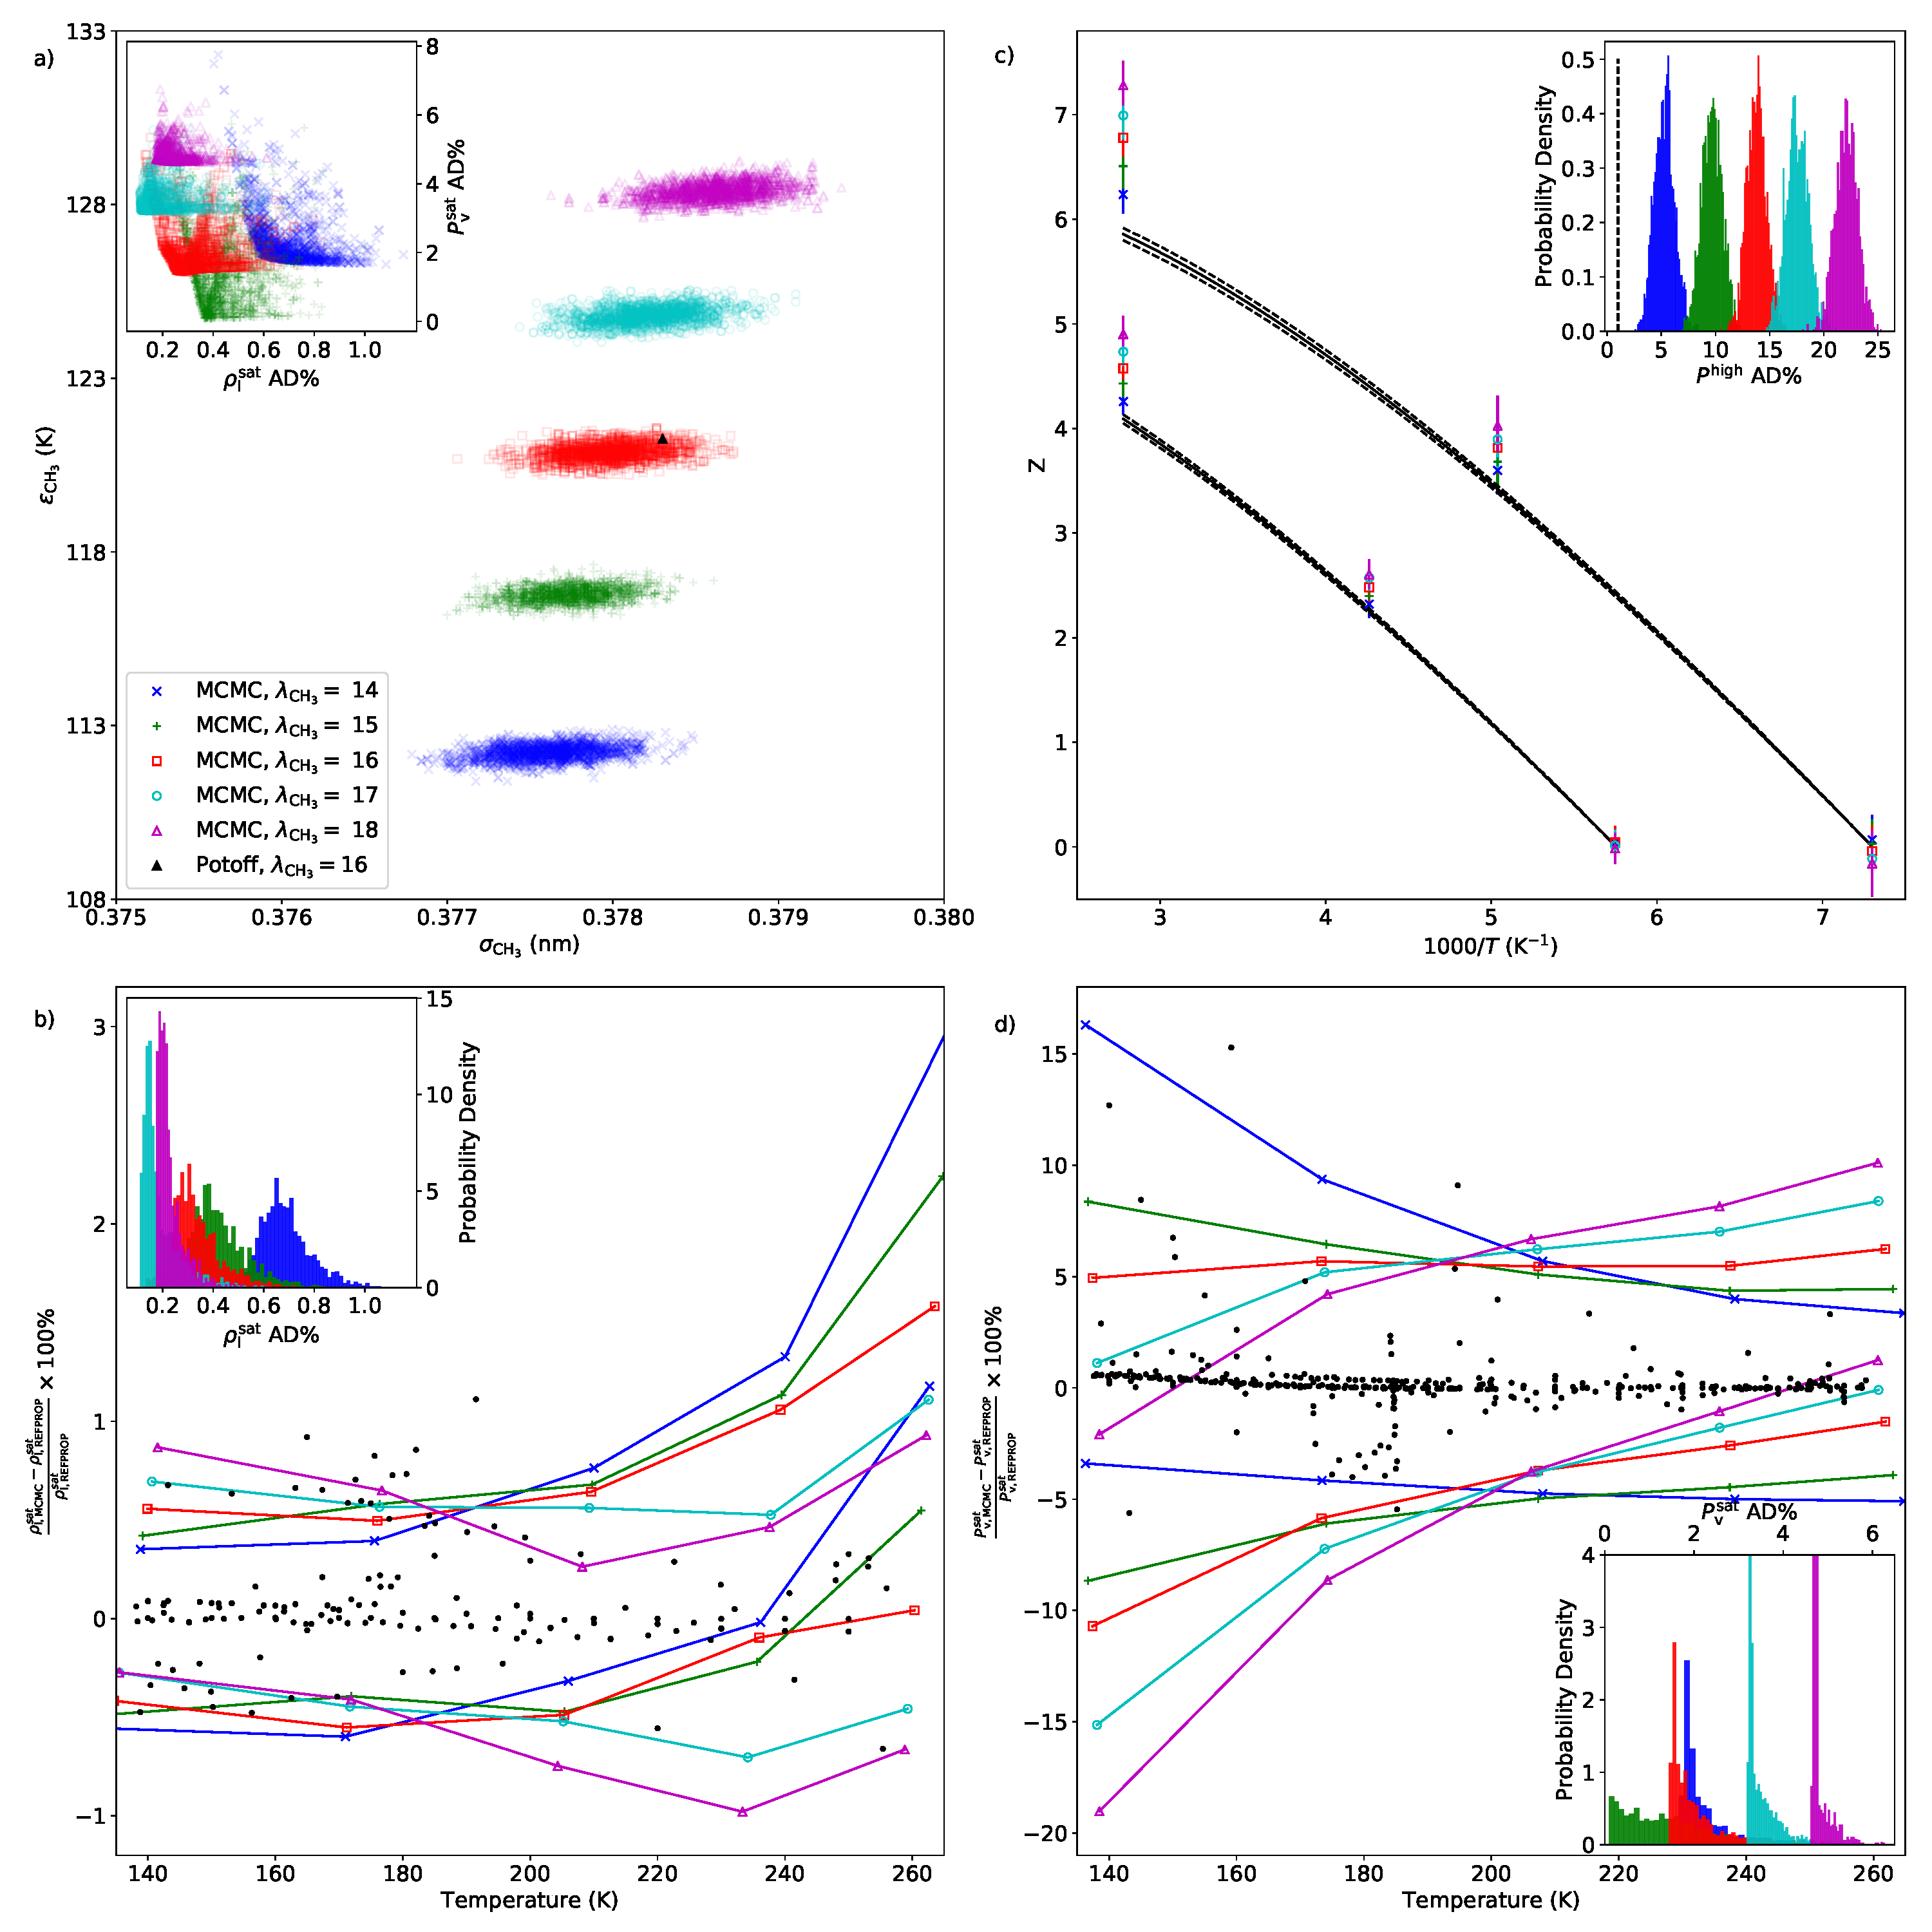
\includegraphics[width=6.4in]{MCMC_Mie_14_15_16_17_18_ethane_alt2}
	\caption{MCMC results confirm that the UA Mie $\lambda$-6 potential cannot adequately predict both VLE and high pressures for supercritical fluids and compressed liquids.  Potoff parameter set is provided in Panel a) as a reference for $\lambda_{\rm CH_3} = 16$. REFPROP uncertainty in $P^{\rm high}$ is $\pm 1$\%. Experimental data used to compute the likelihood are included in Panels b) and d) as black dots.}
	\label{fig:MCMC_Mie_14_15_16_17_18_ethane}
\end{figure} 

Panel a) in Figure \ref{fig:MCMC_Mie_14_15_16_17_18_ethane} demonstrates that $\epsilon_{\rm CH_3}$ depends more strongly than $\sigma_{\rm CH_3}$ on $\lambda_{\rm CH_3}$. Panel b) with the corresponding inset demonstrates that the best prediction of $\rho_{\rm l}^{\rm sat}$ is obtained for higher values of $\lambda_{\rm CH_3}$. Panel d) demonstrates that the 14-6 and 18-6 potentials over- and under-predict $P_{\rm v}^{\rm sat}$ at low temperatures, respectively, while the 15-6 potential demonstrates the least amount of bias and the lowest AD\% (see inset) in $P_{\rm v}^{\rm sat}$. The inset of Panel a), helps to visualize the overall performance of different values of $\lambda_{\rm CH_3}$. Notice the Pareto front (i.e. the trade-off) between the two properties included in the objective function, namely, $\rho_{\rm l}^{\rm sat}$ and $P_{\rm v}^{\rm sat}$. Consistent with the insets of Panels b) and d), the 15-6 potential has the lowest AD\% in $P_{\rm v}^{\rm sat}$ while the 16-6, 17-6, and 18-6 have slightly better AD\% in $\rho_{\rm l}^{\rm sat}$. Finally, Panel c) demonstrates that all of the sampled $\epsilon_{\rm CH_3, MCMC}$ and $\sigma_{\rm CH_3, MCMC}$ parameter sets for different values of $\lambda_{\rm CH_3}$ over-predict $Z$ at high temperatures and densities. This supports the claim for the present manuscript, namely, that the UA Mie $\lambda$-6 potential cannot adequately predict both VLE and high pressures for supercritical fluids and compressed liquids. As expected, the larger the value of $\lambda_{\rm CH_3}$, the greater the force field over-predicts $P^{\rm high}$. For example, the 15-6 and 16-6 potentials, which are the two best potentials based on VLE, over-predict $P^{\rm high}$ by around 10 and 15\%, respectively. 

While the 14-6 potential only demonstrates a 5\% disagreement in $P^{\rm high}$ (notice that the REFPROP deviation is only 1\%), the deprecation in the quality of VLE is significant. This can be quantified by determining the Bayes factor for different values of $\lambda_{\rm CH_3}$ (normalized by the 14-6 potential). Figure \ref{fig:Evidence_Mie_CH3_CH2} Panel a) shows that the 15-6 and 16-6 potentials are equally justified while the evidence for 14-6 and 17-6 is much less and the evidence for 18-6 is negligible. Although the Bayes factors in Figure \ref{fig:Evidence_Mie_CH3_CH2} and Table \ref{tab:Bayes_Factors} for the 15-6 and 16-6 are not as large as are typically reported, note that these results are based on the VLE data and the error model. We have chosen a very conservative error model to demonstrate the inadequacy in predicting $P^{\rm high}$. However, a less conservative error model would provide more convincing evidence for the Bayes factors. Also, recall that ITIC is limited to $T^{\rm sat} < 0.85 T_c$. Therefore, it is possible that the optimal value of $\lambda_{\rm CH_3}$ could be deduced (i.e. larger Bayes factors) if higher temperature VLE data were included (say from 260-290 K). Based on the observed bias in $\rho_{\rm l}^{\rm sat}$ at higher temperatures (240-260 K) for the 14-6 potential, it appears that these data would strengthen the claim that the 14-6 potential should not be used for VLE. It is unclear whether higher temperature data would support the 15-6 or 16-6 potential more, likely the optimal $\lambda_{\rm CH_3}$ value is some fraction between 15 and 16.

\begin{figure}[htb!]
	\centering
	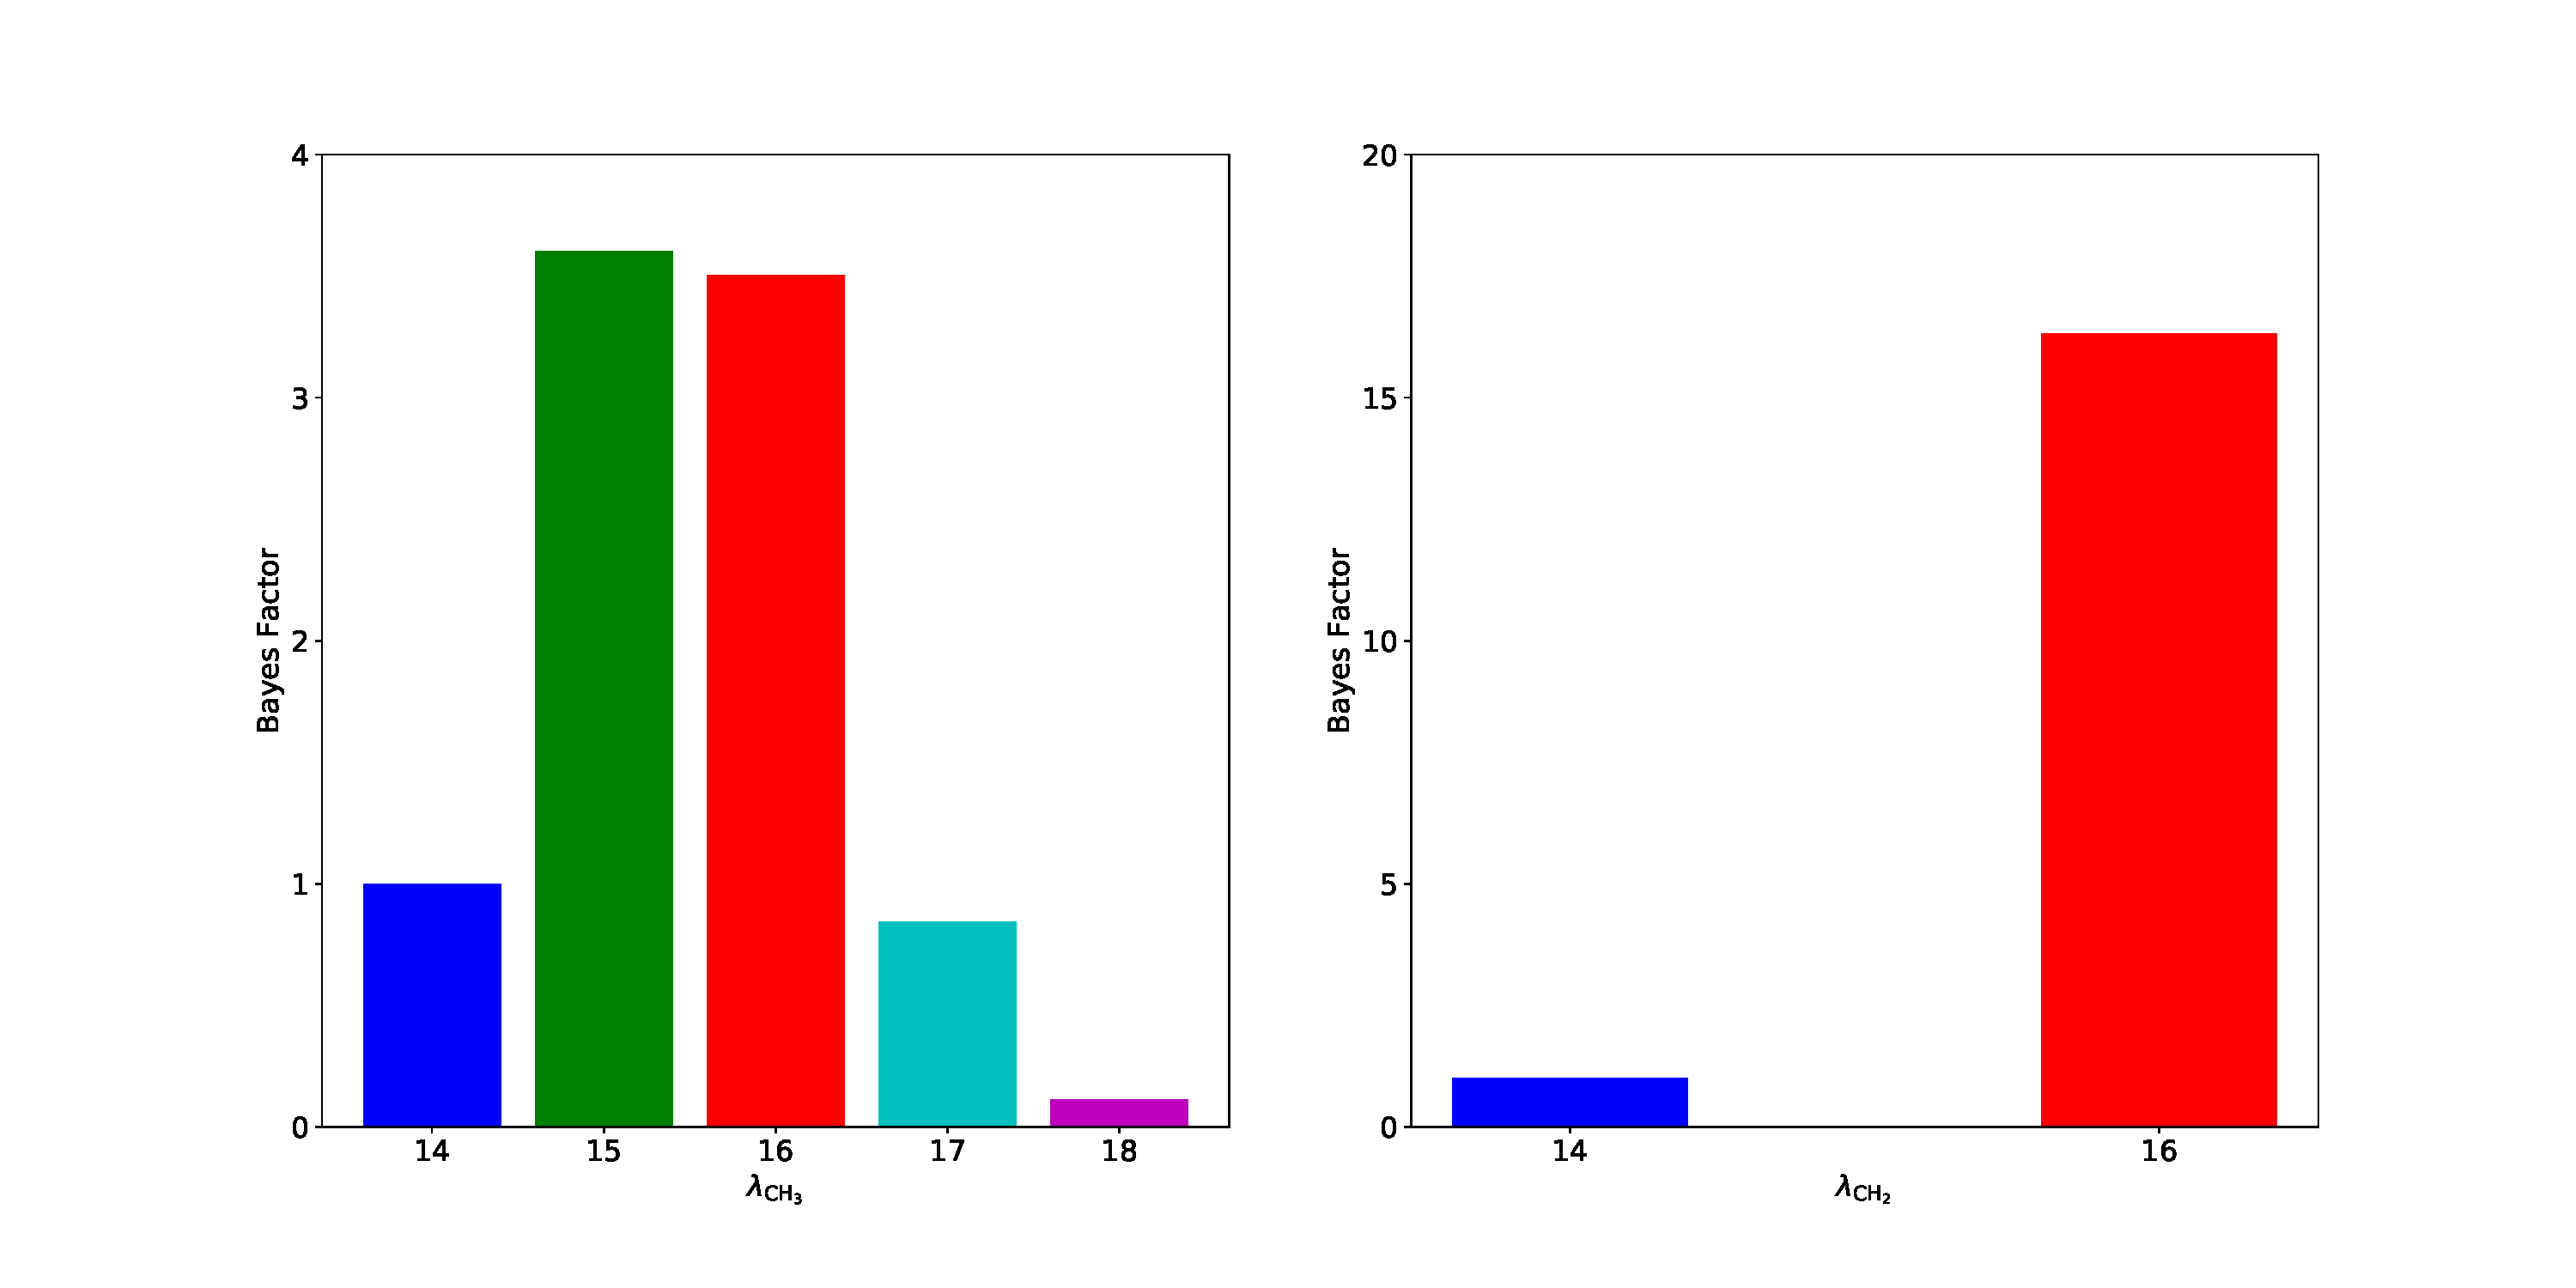
\includegraphics[width=6.4in]{Evidence_Mie_CH3_CH2}
	\caption{Evidence in Panel a) supports the UA Mie 15-6 and 16-6 potentials for ethane (CH$_3$) almost equally. Evidence in Panel b) strongly supports $\lambda_{\rm CH_2} = 16$ over $\lambda_{\rm CH_2} = 14$ for propane and \textit{n}-butane.}
	\label{fig:Evidence_Mie_CH3_CH2}
\end{figure}

\begin{table}[h!]
	\caption{Bayes factors for different values of $\lambda$ (normalized by $\lambda= 14$).} \label{tab:Bayes_Factors}
	\begin{center}
		\begin{tabular}{|c|c|c|}
			\hline
			$\lambda$ & CH$_3$ & CH$_2$ \\ \hline
			14 & 1.0 & 1.0 \\ 
			15 & 3.6 & - \\  
			16 & 3.5 & 16.3 \\ 
			17 & 0.8 & - \\ 
			18 & 0.1 & - \\  
			\hline
		\end{tabular}
	\end{center} 
\end{table}

\subsection{Larger \textit{n}-alkanes} \label{Larger_nalkanes}

Figure \ref{fig:MCMC_Mie_14_16_propane_butane_octane} presents the MCMC sampled $\epsilon_{\rm CH_2}$ and $\sigma_{\rm CH_2}$ parameter sets with Panels a) and b) corresponding to $\lambda_{\rm CH_2} = 16$ and $\lambda_{\rm CH_2} = 14$, respectively. Panel a) contains the MCMC parameter sets for propane, \textit{n}-butane, and \textit{n}-octane, while Panel b) contains results for propane and \textit{n}-butane. Figure \ref{fig:MCMC_Mie_14_16_propane_butane_octane} also includes contours of the average percent deviations (AD\%) in $P^{\rm high}$ relative to the REFPROP correlations, with the ``REFPROP uncertainty'' region corresponding to AD\% of $\pm 1$.

\begin{figure}[htb!]
	\centering
	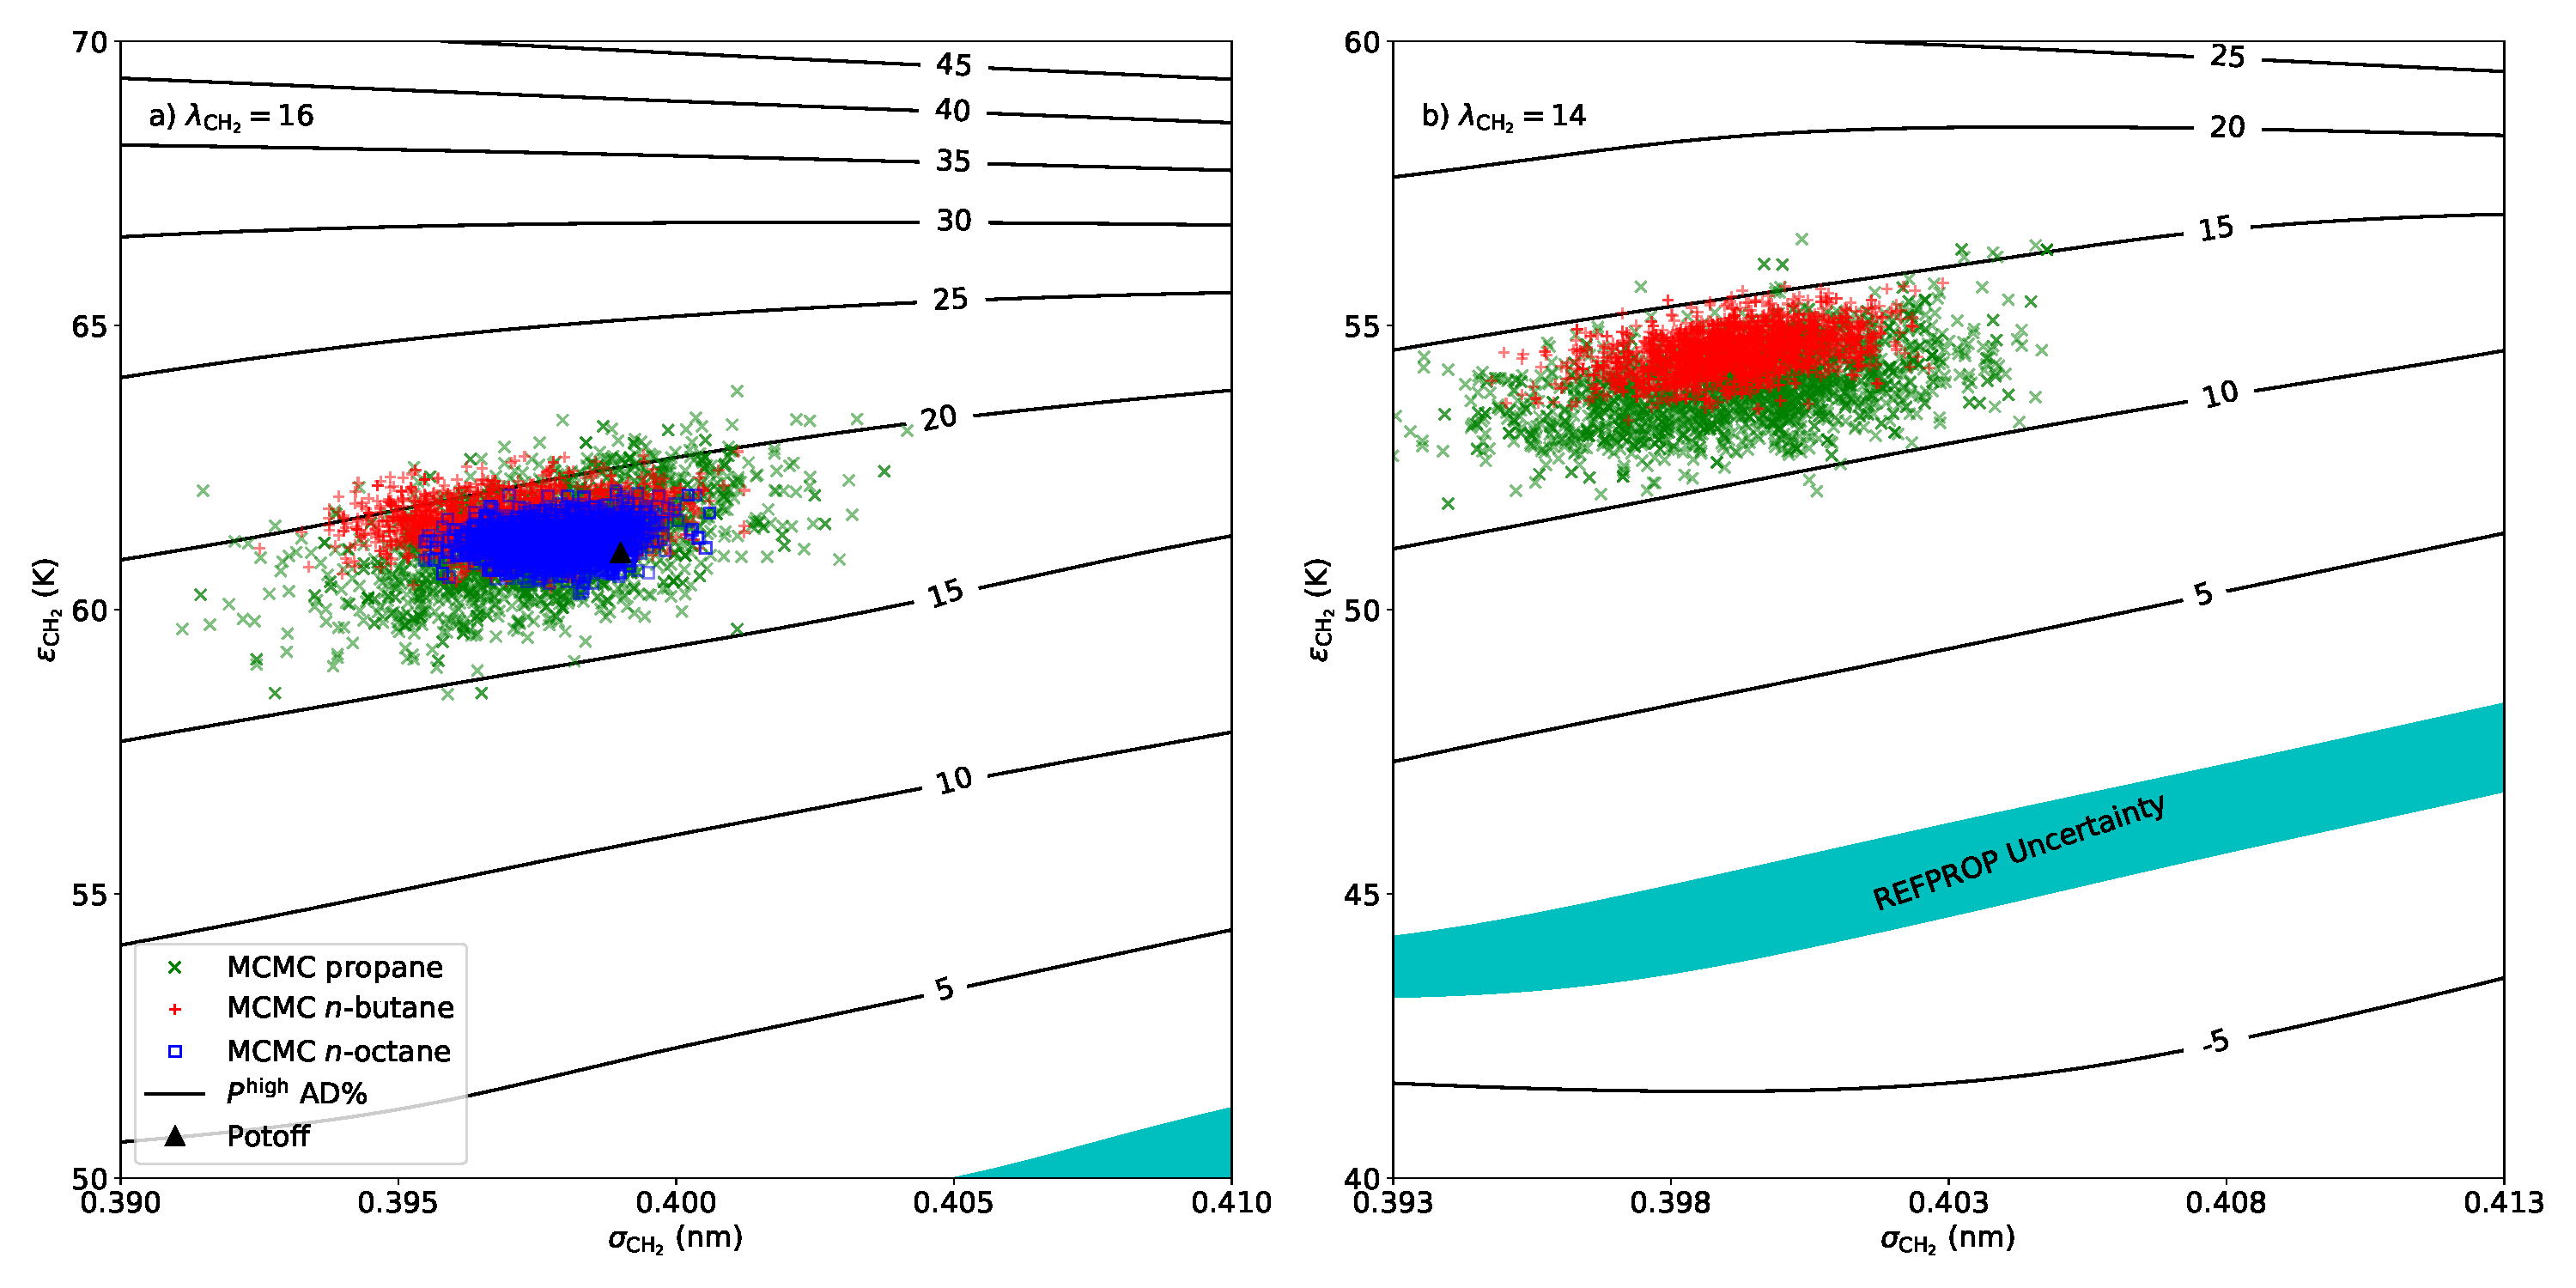
\includegraphics[width=6.4in]{MCMC_Mie_14_16_propane_butane_octane}
	\caption{MCMC sampled $\epsilon_{\rm CH_2}$ and $\sigma_{\rm CH_2}$ parameter sets result in large AD\% for $P^{\rm high}$. Panels a) and b) correspond to $\lambda_{\rm CH_2} = 16$ and $\lambda_{\rm CH_2} = 14$, respectively. REFPROP uncertainty in $P^{\rm high}$ is $\pm 1$\%. Potoff parameter set is provided as a reference for $\lambda_{\rm CH_2} = 16$.}
	\label{fig:MCMC_Mie_14_16_propane_butane_octane}
\end{figure} 

%Figure \ref{fig:MCMC_Mie16_propane_butane_octane} presents the MCMC sampled $\epsilon_{\rm CH_2}$ and $\sigma_{\rm CH_2}$ parameter sets with $\lambda_{\rm CH_2} = 16$. Notice that the MCMC sampled $\epsilon_{\rm CH_2}$ and $\sigma_{\rm CH_2}$ parameter sets overlap considerably for propane, \textit{n}-butane, and \textit{n}-octane. This supports the common assumption of transferability of CH$_2$ parameters between different \textit{n}-alkanes. Note that the uncertainty in the parameters is largest for propane and smallest for \textit{n}-octane. This suggests that, as expected, the sensitivity of $\rho_{\rm l}^{\rm sat}$ and $P_{\rm v}^{\rm sat}$ with respect to the CH$_2$ parameters increases with increasing number of CH$_2$ interaction sites. Also, notice that the Potoff parameter set is within the MCMC sample region. More importantly, for the purposes of this manuscript, the MCMC sampled $\epsilon_{\rm CH_2}$ and $\sigma_{\rm CH_2}$ parameter sets have $P^{\rm high}$ AAD\% $\approx 16$-$23$, while the REFPROP uncertainty in $P^{\rm high}$ is estimated to be around $1$\%.

%\begin{figure}[htb!]
%	\centering
%	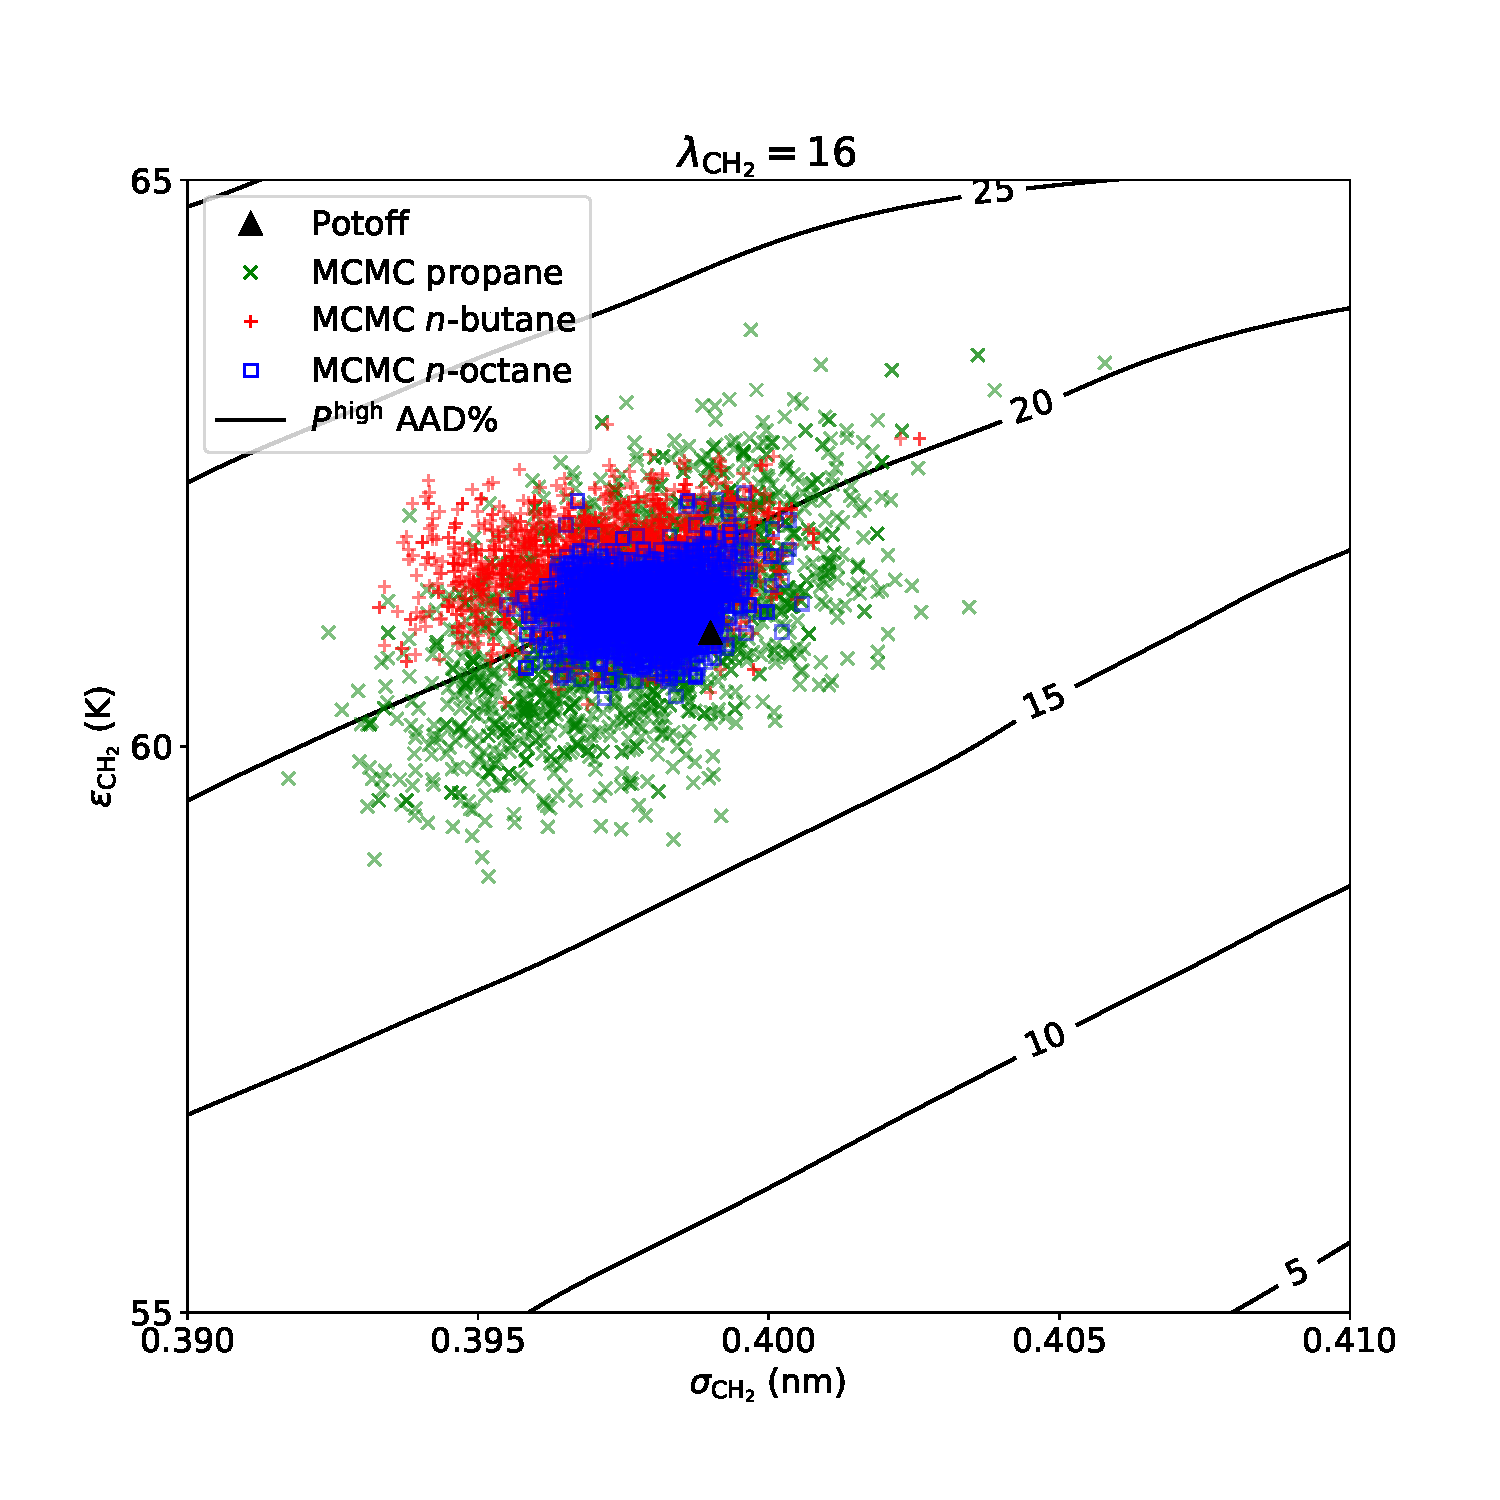
\includegraphics[width=3.2in]{MCMC_Mie16_propane_butane_octane}
%	\caption{MCMC sampled $\epsilon_{\rm CH_2}$ and $\sigma_{\rm CH_2}$ parameter sets with $\lambda_{\rm CH_2} = 16$ result in AAD\% $\approx 16$-$23$ for $P^{\rm high}$. REFPROP uncertainty in $P^{\rm high}$ is $\pm 1$\%. Potoff parameter set is provided as a reference.}
%	\label{fig:MCMC_Mie16_propane_butane_octane}
%\end{figure}

Notice in Figure \ref{fig:MCMC_Mie_14_16_propane_butane_octane} that the MCMC sampled $\epsilon_{\rm CH_2}$ and $\sigma_{\rm CH_2}$ parameter sets, for a given value of $\lambda_{\rm CH_2}$, overlap considerably for the different compounds. This supports the common assumption of transferability of CH$_2$ parameters between different \textit{n}-alkanes. Also, note that the uncertainty in the parameters is largest for propane and smallest for \textit{n}-octane. This suggests that, as expected, the sensitivity of $\rho_{\rm l}^{\rm sat}$ and $P_{\rm v}^{\rm sat}$ with respect to the CH$_2$ parameters increases with increasing number of CH$_2$ interaction sites. Notice, in Panel a), that the Potoff parameter set for $\lambda_{\rm CH_2} = 16$ is within the MCMC sample region.

More importantly, for the purposes of this manuscript, the MCMC sampled $\epsilon_{\rm CH_2}$ and $\sigma_{\rm CH_2}$ parameter sets have large AD\% in $P^{\rm high}$. Specifically, $\lambda_{\rm CH_2} = 16$ and $\lambda_{\rm CH_2} = 14$ have, respectively, AD\% of $\approx 16$-$21$ and $\approx 10$-$15$, much greater than the REFPROP uncertainty of around $1$\%. Because the ``REFPROP uncertainty'' contours are roughly parallel to the MCMC region and found at much lower $\epsilon_{\rm CH_2}$ (around 45 K for $\sigma_{\rm CH_2} = 0.399$ nm), in order to accurately predict $P^{\rm high}$, it is necessary to sacrifice accuracy in $\rho_{\rm l}^{sat}$ and $P_{\rm v}^{\rm sat}$. This suggests that neither the UA Mie 16-6 or 14-6 models are capable of predicting VLE and $PVT$ for supercritical fluids and compressed liquids of \textit{n}-alkanes. Finally, although the UA Mie 14-6 AD\% is slightly better than the UA Mie 16-6 AD\%, the UA Mie 14-6 is significantly less reliable for VLE. Figure \ref{fig:Evidence_Mie_CH3_CH2} Panel b) and Table \ref{tab:Bayes_Factors} demonstrate the strong evidence for a 16-6 potential over a 14-6 potential based on VLE data. (The evidence for CH$_2$ is likely stronger than CH$_3$ because VLE data from more than one compound were included.) Therefore, considering the deprecation in VLE, the marginal gain in accuracy for $P^{\rm high}$ likely does not merit using a UA Mie 14-6 potential.

% Therefore, Figure \ref{fig:MCMC_Mie_14_16_propane_butane_octane} provides convincing evidence that, regardless of the value of $\lambda$, the UA Mie $\lambda$-6 model is not capable of predicting both VLE and $PVT$ at high pressures.

%The REFPROP uncertainty region that corresponds to AAD\% of $\pm 1$ is parallel to the MCMC region and found at much lower $\epsilon_{\rm CH_2}$ (around 45 K for the same $\sigma_{\rm CH_2}$). Therefore, in order to accurately predict $P^{\rm high}$, it is necessary to sacrifice accuracy in $\rho_{\rm l}^{sat}$ and $P_{\rm v}^{\rm sat}$. Figures \ref{fig:MCMC_Mie16_propane_butane_octane}-\ref{fig:MCMC_Mie14_propane_butane} provide convincing evidence that, regardless of the value of $\lambda$, the UA Mie $\lambda$-6 model is not capable of predicting both VLE and $PVT$ at high pressures.

%Also, notice that the MCMC sampled $\epsilon_{\rm CH_2}$ and $\sigma_{\rm CH_2}$ parameter sets overlap considerably for the two compounds. In other words, the $\epsilon_{\rm CH_2}$ and $\sigma_{\rm CH_2}$ parameter sets for propane and \textit{n}-butane are indistinguishable to within uncertainty. This supports the common assumption of transferability of CH$_2$ parameters between different \textit{n}-alkanes.

%Figure \ref{fig:MCMC_Mie16_propane_butane_octane} suggests that the UA Mie 16-6 potential is not capable of predicting VLE and $PVT$ for supercritical fluids and compressed liquids of propane, \textit{n}-butane, and \textit{n}-octane. Figure \ref{fig:MCMC_Mie14_propane_butane} demonstrates that the UA Mie 14-6 potential is also not capable of predicting both properties for propane and \textit{n}-butane. Specifically, all of the MCMC sampled $\epsilon_{\rm CH_2}$ and $\sigma_{\rm CH_2}$ parameter sets in Figure \ref{fig:MCMC_Mie14_propane_butane} have $P^{\rm high}$ AAD\% $\approx 10$-$15$. Although this is improvement relative to the UA Mie 16-6 AAD\%, recall that the UA Mie 14-6 is less reliable for VLE. Therefore, considering the significant deprecation in VLE, the marginal gain in accuracy for $P^{\rm high}$ likely does not merit using a UA Mie 14-6 potential. 
%
%Figure \ref{fig:MCMC_Mie14_propane_butane} also includes the ``REFPROP uncertainty'' region which corresponds to AAD\% of $\pm 1$.  Because the ``REFPROP uncertainty'' contours are parallel to the MCMC region and found at much lower $\epsilon_{\rm CH_2}$ (around 45 K for the same $\sigma_{\rm CH_2}$), in order to accurately predict $P^{\rm high}$, it is necessary to sacrifice accuracy in $\rho_{\rm l}^{sat}$ and $P_{\rm v}^{\rm sat}$. Figures \ref{fig:MCMC_Mie16_propane_butane_octane}-\ref{fig:MCMC_Mie14_propane_butane} provide convincing evidence that, regardless of the value of $\lambda$, the UA Mie $\lambda$-6 model is not capable of predicting both VLE and $PVT$ at high pressures.

%\begin{figure}[htb!]
%	\centering
%	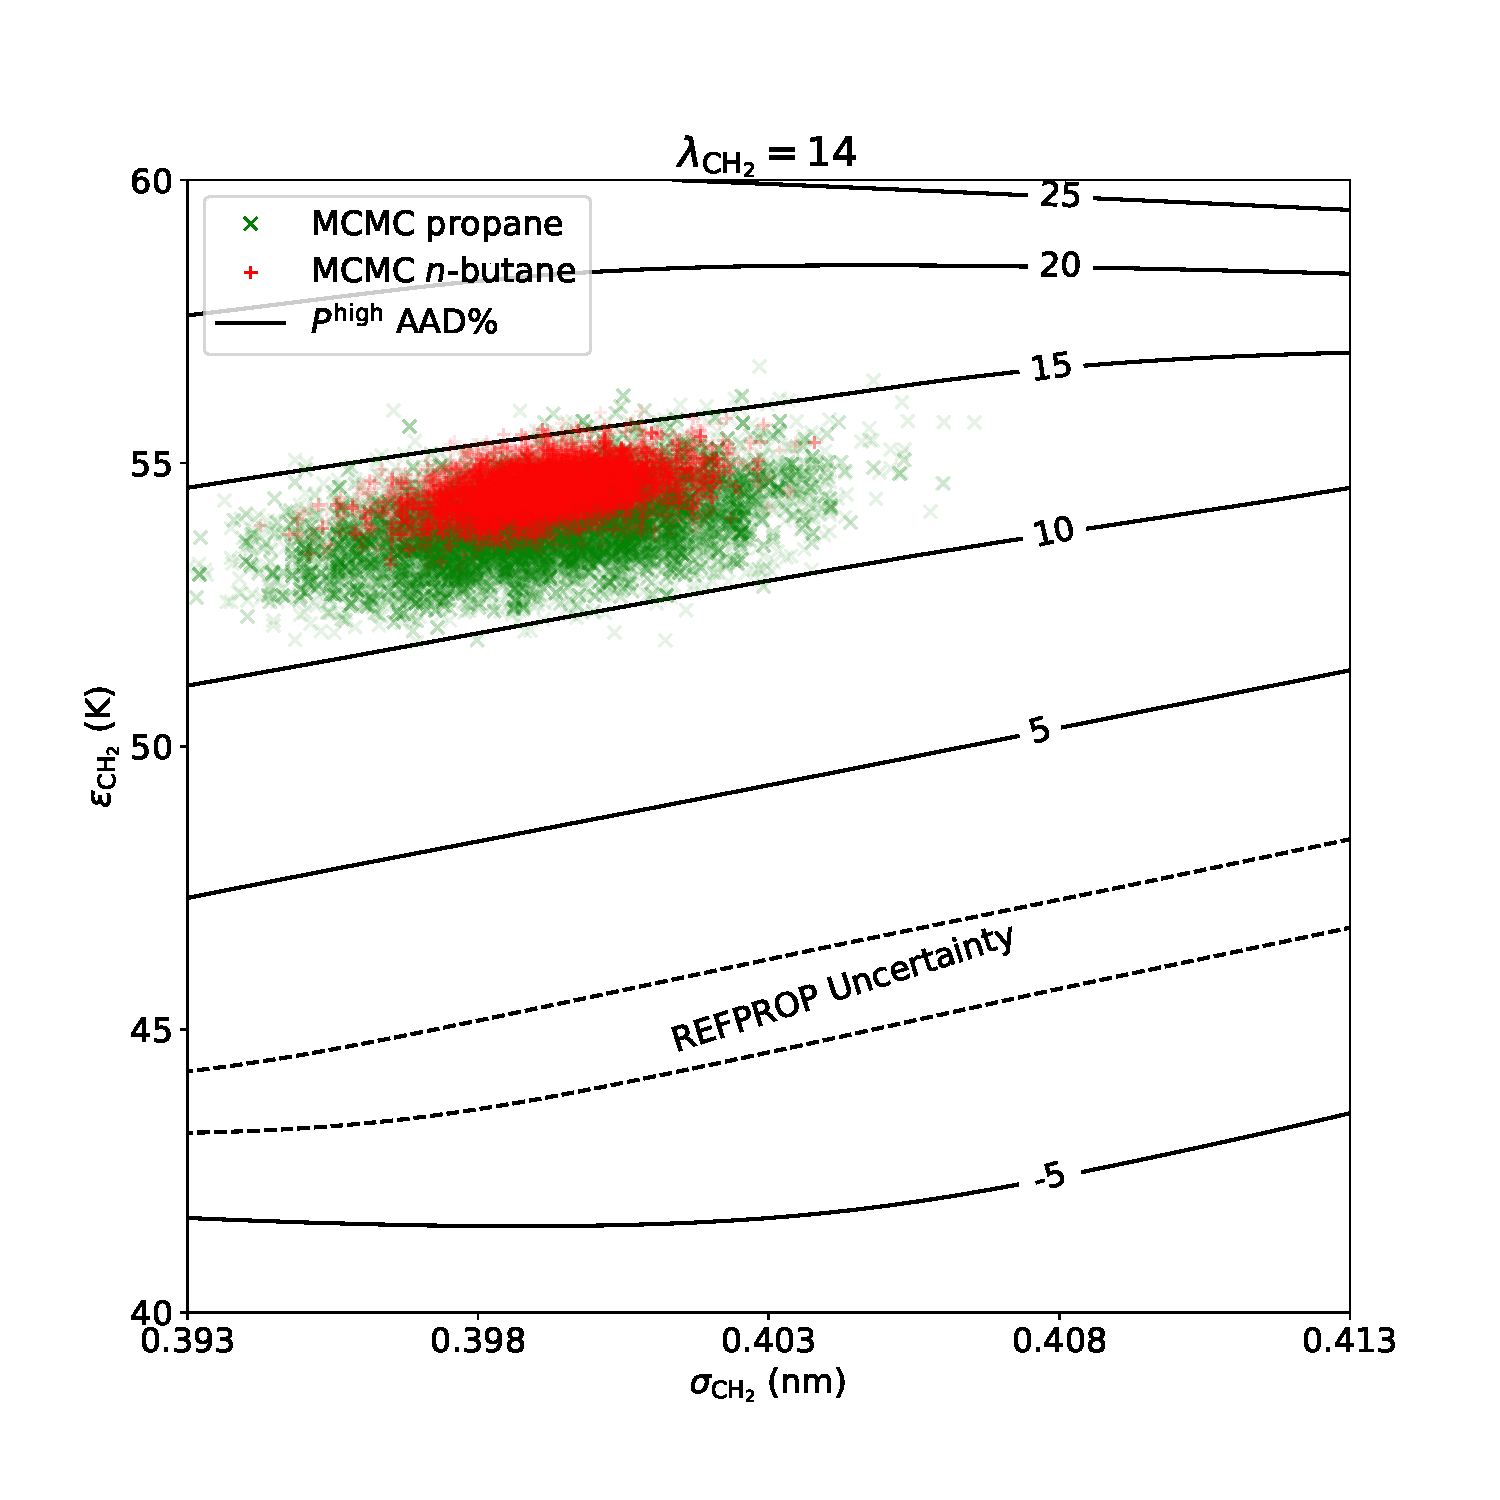
\includegraphics[width=3.2in]{MCMC_Mie14_propane_butane}
%	\caption{MCMC sampled $\epsilon_{\rm CH_2}$ and $\sigma_{\rm CH_2}$ parameter sets with $\lambda_{\rm CH_2} = 14$ result in AAD\% $\approx 10$-$15$ for $P^{\rm high}$. REFPROP uncertainty in $P^{\rm high}$ is included at $\pm 1$\%.}
%	\label{fig:MCMC_Mie14_propane_butane}
%\end{figure}

%\begin{enumerate}
%	\item Figure: The uncertainty regions for CH3, CH2, CH, and C. I can include 14-6, 15-6, and 16-6. Perhaps I will only do this rigorous analysis for CH3 or for CH3 and CH2. Probably not for all. 
%%MRS: might be weaker to say it's a rigorous bayesian analysis if only done for 2; people could always say ``but maybe it will work for C and CH'', though obviously, it C and CH parmeters are irrelevant for n-alkanes.  
%%MRS: so one could optimize CH3 and CH2, and then optimize for C and CH given CH2 and CH3. Importantly, you can back-calcuate the confidence regions for different CH2 and CH3 parameters for n-alkanes, alone, since that just affects the posteriors when adding C and CH data.  
%%MRS: is the reason not for all the computational expense?
%%MRS: it could be with the constraints on CH2 and CH3 from the n-alkanes, you can do a restricted 3D search with CH (not bothering to do already low probability regions of CH3 and CH3, and then do a restricted 4D search with the constraints on CH3/CH2/CH''.  Not many molecules that have C and CH, so fewer simulations to do.  
%%MRS: or could just say ``doesn't work for normal, so no point in worrying about C and CH''.
%I could include the results from the alternative posterior (excluding Pvsat and including high pressures) but then it might be out of place in this section.
%	\item Bayes factors demonstrate that, for VLE, a 15-6 or 16-6 potential are favored significantly more than a 14-6 (could include 17-6 or 18-6 as well)
%%MRS: probably want to go until the probability turns down again. 
%	\item CH2 credible regions overlap considerably between propane, n-butane, and n-octane
%%MRS: You want to show the combined region as well, though; muliplying the probabilities. 
%%MRS: Do you want to include data showing that separate CH2 and CH3 parameters are necessary? Would be nice to use Bayesian analysis to show more dimensions are necessary. Is that already established?  Might be a nice way to demonstrate Bayesian approach to show things already established like this.
%	\item By comparing the Bayes factor of a transferable CH2 site and three independent CH2 sites we observe that the CH2 sites are indistinguishable
%	\item Statement about CH credible regions for isobutane, isopentane, and isohexane
%	\item Statement about C credible region for isooctane and neopentane
%\end{enumerate}

%\subsection{Propagation of uncertainties}

% I am not sure where this should go. Perhaps supporting information?
%\begin{enumerate}
%%MRS: be more precise about what you mean by propagation of uncertainties. 95% confidence intervals?  Standard deivations? What is the point that you are proving with this data?
%	\item Figure: Uncertainties in rholsat and Pvsat for n-alkanes. Include 14-6, 15-6, 16-6.
%	\item Figure: Uncertainties in rholsat and Pvsat for branched alkanes. Include only 16-6.
%	\item Clearly the uncertainties are fairly conservative due to the relatively large numerical uncertainties we assigned in the posterior
%%MRS: Not clear; uncertainties in rholsat and Pvsat affect the posterior . . . ? Important point; the way that we've defined likelihood includes the experimental uncertainty, but not the numerical uncertainty. 
%	\item Figure: Z vs 1000/T for n-alkanes where the error bars represent the Bayesian uncertainties from VLE. Include 14-6, 15-6, and 16-6 results.
%%MRS: for the points below, what is the proof of the points; the figure of Z vs 1000/T? Be clear.
%	\item The 16-6 potential is not able to predict both VLE and compressed liquid/supercritical pressures
%	\item VLE is much worse for 14-6, about the same for 15-6
%	\item Condensed liquid pressures are slightly better for 14-6 and 15-6 but still over-predict
%	\item Figure: Z vs 1000/T for branched alkanes. Results are only included for the 16-6 potential.
%	\item Same results as for normal alkanes.
%\end{enumerate}

%%% RAM: We feel like this discussion could just be a paragraph saying that if Pvsat is not important you could use a 14-6 potential and match just liquid phase pressures
%\subsection{Optimal $\lambda$ for high pressures}
%MRS: might need to justify why or why not would would need Pvstat.
%\begin{enumerate}
%	\item We modify the posterior by excluding the Pvsat data and including the REFPROP correlations at high pressures
%	\item Figure: I can either include the parameter uncertainties here or back in the Parameter Uncertainties section. I could even move this to supporting information
%	\item Bayes ratios show the evidence for different values of $\lambda$
%	\item We recommend that lower values of $\lambda$ be favored
%%MRS: but the thesis is that MIE isn't sufficient; difficult if you are complicating the thesis too much.
%\end{enumerate}

\section{Recommendations and Limitations}

Note that the simulation values used by Thol et al. were derivatives of the residual Helmholtz free energy $(\partial^n a^{\rm r})$ with respect to inverse temperature and/or density \cite{Thol2016_siloxane_first,Thol2016_siloxane,Thol2017}, while in this study we simply compare the $PVT$ behavior. Aside from the advantage of simplicity (most simulation packages do not provide $\partial^n a^{\rm r}$), this choice is based on the fact that $PVT$ is more readily understood and easier to visualize. In other words, it is easier to quantify the impact on process design caused by deviations in $PVT$ behavior than derivatives in the residual Helmholtz free energy. Furthermore, as demonstrated by Thol et al., an inaccurate prediction of some $\partial^n a^{\rm r}$ does not necessarily result in poor prediction of $PVT$ behavior or heat capacities \cite{Thol2016_siloxane_first}. It is important to remember that $PVT$ depends only on the first derivative of Helmholtz free energy with respect to density. Therefore, future work should investigate the adequacy of force fields to predict heat capacities, which depend on temperature derivatives, at higher temperatures and pressures. We would like to emphasize that, although we did not use $\partial^n a^{\rm r}$ for our analysis, including higher order derivatives of the residual Helmholtz free energy from molecular simulation has significant advantages for developing FEOS as it eliminates redundant information found in traditional macroscopic properties \cite{Thol2016_LJ,Thol_LJTS,Rutkai2017,Lustig2015,Rutkai2013,Rutkai2015}.

% is a significant advantage of the approach implemented by Thol et al. for FEOS development.

%\section{Future Work}
%%MRS: I don't think there's that good motivation for ``future work'' sections in general. Either make AUA part of the thesis, or don't include them.  There can be discussion of possible alternatives. 
%\begin{enumerate}
%	\item As observed in the case study, the AUA approach typically provides more reliable estimates at high pressures.
%	\item At higher pressures you need the hydrogens, the higher the shift in the bond-length the better.
%	\item For example, notice that the AUA LJ (TraPPE-2) model is better than the AUA Mie (TAMie) and AUA Exp-6 (ErrExp-6), despite having fewer fitting parameters. This is because they use a much larger bond displacement.
%	%%% RAM: I do not have results for AUA4, do I really need all of these examples from the literature?
%        %%% MRS: depends on the thesis. . .  
%	\item An alternative method to AUA is to use an extended Lennard-Jones potential, 12-10-8-6, that has the flexibility of a Mie potential but without the steep barrier
%\end{enumerate}
 
\section{Conclusions} \label{Conclusions}

Recently, molecular simulation results at extreme temperatures and pressures have been used to supplement experimental data when developing a fundamental equation of state. As discussed by Thol et al., due to uncertainties and deficiencies in the force field, experimental data should be favored over molecular simulation values whenever possible. However, in principle, a FEOS could be developed for compounds without any experimental data by using only molecular simulation results, if the force field were reliable and transferable over different $PVT$ conditions. In part, one of our aims was to determine whether the united-atom Mie $\lambda$-6 potential for normal and branched alkanes was reliable enough that a FEOS could be developed strictly from molecular simulation results. Unfortunately, the Bayesian statistical analysis performed in this study suggests that this model type (UA Mie $\lambda$-6) is not adequate for predicting \textit{both} VLE properties and high pressures for supercritical fluids and compressed liquids. Specifically, no set of $\epsilon$, $\sigma$, and $\lambda$ can adequately predict VLE and PVT behavior. Therefore, we recommend that alternative models be considered for developing FEOS, such as force fields using anisotropic-united-atom, all-atom, and/or alternative non-bonded potentials, e.g. Buckingham exponential-6, extended Lennard-Jones, etc.

%   The aim of the present study was to determine whether the Mie potential is a candidate for supplanting experimental data by accurately predicting both VLE properties and pressures for supercritical fluids and compressed liquids. 
%
%The results from this study suggest that the united-atom Mie $\lambda$-6 potential is not adequate for predicting both VLE properties and pressures for supercritical fluids and compressed liquids of normal and branched alkanes.

%\begin{enumerate}
%%MRS: make claims more specific: you said Mie not good for VLE - did you mean that its's good for low pressure VLE, but not high pressure?
%%	\item Although the UA Mie potential provides great improvement over the UA LJ 12-6 potential for VLE, it drastically over-predicts pressures for supercritical fluids and compressed liquids (actually for supercritical fluids it over-predicts at high densities and under-predicts at low densities. Not sure I want to open up that can of worms.)
%%%MRS: if you've observed it, should mention it. 
%%	\item By performing a rigorous statistical analysis, we verify that no set of $\epsilon$ and $\sigma$ can adequately predict VLE and high pressures (I need a better way to refer to this) for a 16-6, 15-6, or 14-6 potential.
%%MRS: Are those two different things: ``VLE'' and ``high pressures'', or is it just ``high pressure properties, including VLE and supercritical densities''.
%\end{enumerate}

%%% This was taken from previous drafts of the first manuscript. These paragraphs will probably not go in this manuscript.
%%%% The next few paragraphs probably belong in Part II where we focus on parameterization. I think it suffices in this paper to just say that we need surrogate models for computational reasons.

%%% Some of this discussion actually belongs in the publication that I do with Elliott and Potoff most likely

%The increase in the number of model parameters causes the parameterization to be more difficult, especially when direct molecular simulations are required. For example, the Mie $\lambda$-6 parameters reported by Potoff are obtained by scanning the parameter space using predefined grid spacing. Although this scanning approach is useful for verifying that a global minimum is found, it scales as $O(n_g^{n_p})$ where $n_g$ is the number of grid points per $n_p$ and $n_p$ is the number of parameters. With $n_g \approx 30$ performing molecular simulations at each grid point becomes computationally intractable for $n_p > 3$. This is also problematic for performing a Pareto front \cite{Pareto_Deriv,Pareto_LJPQ,Pareto_ST} or feasible region \cite{Mess4} analysis that typically require a very refined grid of the parameter space. Furthermore, Bayesian methods that use Markov Chain Monte Carlo (MCMC) to sample from the parameter space become extremely expensive in higher dimensions when direct simulations are required at each step \cite{Bay_UQ,Bay_Deriv,Bay_MD}. 
%%% This may not be true. Higher dimensional optimizations actually are less likely to get trapped, apparently.
%A common problem for any high dimensional parameter space is that gradient based optimizations can get trapped in local minima while so-called global optimizations may require inordinate number of ``function evaluations'' (i.e. molecular simulations). Increasing the number of parameters can also lead to a high degree of parameter correlation. In addition, over-parameterization can result in non-physical optimal parameters which will likely extrapolate poorly. For these reasons, it is common to make model simplifications by reducing the number of parameters in a judicious manner. There are four primary ways to accomplish this: 1) optimizing the intramolecular contribution independent of the intermolecular potential 2) constraining parameters in the non-bonded potential 3) employing combining rules and 4) transferring parameters for similar site types. Unfortunately, each of these model simplifications can lead to model deficiencies.
%
%Typically, intramolecular potentials are obtained by regressing model parameters to match quantum mechanical calculations of different configurations. Subsequently, the intermolecular (non-bonded) potentials are often fit to reproduce experimental data, such as saturated liquid density, vapor pressure, and heat of vaporization. It is commonly assumed that the uncertainty propagated from the intramolecular potential to the vapor-liquid equilibria properties $(\rho_{\rm l}^{\rm sat}, \rho_{\rm v}^{\rm sat}, P_{\rm v}^{\rm sat})$ is negligible relative to the uncertainty caused by the non-bonded potential \cite{Intra_Potoff,Mess4}. Therefore, recent studies that have reported high accuracy force fields have focused primarily on the non-bonded potential (with the main exception being the focus given to anisotropic-united-atoms for terminal sites). For this reason, the present study focuses on parameterizing the non-bonded potential. 
%
%Although the generalized $\lambda_{\rm rep}$--$\lambda_{disp}$ Mie potential (where $\lambda_{\rm rep}$ is the repulsive exponent and $\lambda_{disp}$ is the dispersive exponent) can use any floating point value for $\lambda_{\rm rep}$ and $\lambda_{disp}$, the common practice is to set $\lambda_{disp}=6$. The dispersive tail having an $r^{-6}$ dependence is well founded and should thus lead to improved extrapolation \cite{Mie}. In addition, it is common to only consider integer values of $\lambda_{\rm rep}$ (and sometimes only even integers). This has a nice computational advantage since it is much less expensive to compute a number raised to an integer power than a floating point power \cite{Mie}. Furthermore, this simplifies the optimization to a set of two-dimensional parameter spaces (in $\epsilon$ and $\sigma$) rather than a single three-dimensional parameter space (in $\epsilon, \sigma$, and $\lambda_{\rm rep}$). Unfortunately, this assumption reduces the model flexibility which may lead to inadequate representation of the target variables \cite{Avendano2013}. For example, Papaioannou et al. demonstrated that in many cases the optimal repulsive exponent $(\lambda_{\rm rep})$ is not an integer value \cite{Papaioannou2016}.
%
%Another way to reduce the number of model parameters is by implementing Lorentz-Berthelot (or some other form of) combining rules for cross-interactions. Cross-interaction parameters are the non-bonded parameters for two different site types. Combining rules reduce the number of fitting parameters from being $O(n_i^2)$ to $O(n_i)$, where $n_i$ is the number of site types. In addition, combining rules are intended to ensure that cross-interaction parameters are physically reasonable. That being said, the Lorentz-Berthelot combining rules have been called into question, especially for mixtures \cite{Delhommelle2001}. For this reason, many other \textit{ad hoc} combining rules have been proposed \cite{TraPPEUA2}.
%
%Finally, transferability is an essential assumption in molecular simulation. Transferability assumes that the non-bonded interactions are the same when two chemical moieties are in a similar environment, e.g. the CH$_2$ groups in \textit{n}-butane are the same as the CH$_2$ groups in \textit{n}-pentane. The assumption of transferability has been fundamental to force field development as it allows for a systematic sequential parameterization of functional groups. With this assumption a new chemical moiety is included in the force field by assuming all previous parameters are constant. Therefore, parameterizing the n$^{th}$ site type has the same cost as the first. Unfortunately, validation of transferability is an essential but difficult (and typically omitted) step. 
%
%The primary reason for this is that if two sites are found to not be transferable it may require significant reparameterization of previously optimized site types. For example, the improved TraPPE-UA2 CH$_3$ LJ parameters will likely necessitate reparameterization of other site types from the TraPPE-UA force field that were optimized using the previous TraPPE-UA CH$_3$ LJ parameters. This is an arduous and time-consuming process.
%
%Although the aforementioned simplifications can dramatically reduce the number of fitting parameters, it is not clear \textit{a priori} if these assumptions lead to model inadequacies. In fact, it is almost certain that they do. Ideally, it would be possible to optimize a force field to a large number of data and compounds simultaneously (rather than sequentially) and use rigorous statistical methods to select the optimal non-bonded potentials, validate combining rules, and determine when two sites are in fact transferable. This would require advanced high dimensional optimization routines such as genetic algorithms, leapfrog \cite{RHINEHART2012}, or Bayesian optimizers (see Ucyigitler et al. \cite{SPEADMD}). Unfortunately, these methods are not feasible when molecular simulations are performed at each step of the optimization algorithm. By contrast, Papaioannou et al. and Elliott et al. demonstrated how large amounts of compounds and data can be optimized simultaneously when using less expensive approaches, namely, the SAFT-$\gamma$ equation-of-state and SPEADMD, respectively \cite{Papaioannou2016,SPEADMD}. These methods allowed the authors to determine when additional parameters were needed to distinguish between site types and when two site types were considered indistinguishable.

%% SPEADMD is probably best classified as a configuration sampling based surrogate model

\bibliography{postdoc_references}

\end{document}
